%%%%%%%%%%%%%%%%%%%%%%%%%%%%%%%%%%%%%%%%%
% Simple Sectioned Essay Template
% LaTeX Template
%
% This template has been downloaded from:
% http://www.latextemplates.com
%
% Note:
% The \lipsum[#] commands throughout this template generate dummy text
% to fill the template out. These commands should all be removed when 
% writing essay content.
%%%%%%%%%%%%%%%%%%%%%%%%%%%%%%%%%%%%%%%%%

%----------------------------------------------------------------------------------------
%	PACKAGES AND OTHER DOCUMENT CONFIGURATIONS
%----------------------------------------------------------------------------------------

\documentclass[12pt]{book} % Default font size is 12pt, it can be changed here
	%	\textheight = 30cm
	%	\textwidth = 19cm
		\topmargin = -1cm
		\oddsidemargin = -1cm
		\parindent = 5mm

%\usepackage{geometry} % Required to change the page size to A4
%\geometry{a4paper} % Set the page size to be A4 as opposed to the default US Letter


\usepackage{geometry}
 \geometry{
 a4paper,
 total={150mm,230mm},
 left=25mm,
 top=25mm,
 }



\usepackage{graphicx} % Required for including pictures

\usepackage{float} % Allows putting an [H] in \begin{figure} to specify the exact location of the figure
\usepackage{wrapfig} % Allows in-line images such as the example fish picture




%\usepackage{lipsum} % Used for inserting dummy 'Lorem ipsum' text into the template

\linespread{1.5} % Line spacing

%\setlength\parindent{0pt} % Uncomment to remove all indentation from paragraphs
\usepackage[utf8]{inputenc}
\usepackage[spanish]{babel}
\usepackage[T1]{fontenc}
\usepackage{fancyhdr}
\usepackage{multicol}
\usepackage{cite} % para contraer referencias
% Configurar los encabezados, pies de pagina y paginas de capitulo
% Encabezados
%\lhead[\thepage]{\rightmark}
%\chead[]{}
%\rhead[\thechapter. \leftmark]{\thepage}

\renewcommand{\headrulewidth}{0.4pt}

% Pie de pagina

%\lfoot[]{ITSJR}
\cfoot[]{}
%\rfoot[J.C. Àvila Resendiz]{CICATA}
\renewcommand{\footrulewidth}{0.5pt}
\usepackage{emptypage}

\usepackage{savesym}
\usepackage{amsmath}
\savesymbol{iint}
\usepackage{txfonts}
\restoresymbol{TXF}{iint}

\usepackage[x11names,table]{xcolor}
\usepackage{pstricks}
\usepackage[colorinlistoftodos, textwidth=2cm, shadow]{todonotes}
%\usepackage{hyperref}

\usepackage[colorlinks]{hyperref}
\usepackage[nogroupskip,nopostdot]{glossaries}
\setglossarystyle{altlist}
\makenoidxglossaries

%\usepackage[toc,style=altlistgroup,hyperfirst=false]{glossaries}

\hypersetup{
    colorlinks=true,
    linkcolor=negro,
    filecolor=magenta,      
    urlcolor=blue,
}

\urlstyle{same}

\usepackage{graphicx} % figuras
\usepackage{subfigure} % subfiguras
\usepackage{caption}
\graphicspath{{./imagenes/}} % Specifies the directory where pictures are stored

\definecolor{miorange}{rgb}{0.11, 0.43, 0.21}
\definecolor{negro}{RGB}{35, 0, 0}
\definecolor{blue}{RGB}{0, 0, 255}

%%%%%%%%%%%%%%%%%%%%%%%%%%%%%%%%%%%%%%%%%%%%%%%%%%%%%%%%%%%%%%%%%%%%%%%%%%%%%%%%%%%%%%%%%%%%%%%%%%%%%%%%%%%
%----------------------------------------------------------------------------------------
%	begin {Glosario}
%----------------------------------------------------------------------------------------

\newglossaryentry{SO}{name={SO},description={Es el sistema o conjunto de aplicaciones que permiten que una computadora lleven a cabo sus funciones.}}
\newglossaryentry{Linux}{name={Linux},description={GNU/Linux Sistema Operativo creado y distribuido por miles de 
													personas alrededor del mundo}}
													
\newglossaryentry{Windows}{name={Windows},description={Sistema Operativo creado y distribuido por Microsoft.}}

\newglossaryentry{Mac}{name={Mac},description={Sistema Operativo creado y distribuido por Apple}}

%%%%%%%%%%%%%%%%%%%%%%%%%%%%%%%%%%%%%%%%%%%%%%%%  %%%%%%%%%%%%%%%%%%%%%%%%%%%%%%%%%%%%%%%%%%%%%%%%%%%%%%%%%
\newglossaryentry{}{name={},description={}}
%%%%%%%%%%%%%%%%%%%%%%%%%%%%%%%%%%%%%%%%%%%%%%%%  %%%%%%%%%%%%%%%%%%%%%%%%%%%%%%%%%%%%%%%%%%%%%%%%%%%%%%%%%

%----------------------------------------------------------------------------------------
%	End {Glosario}
%----------------------------------------------------------------------------------------


\pagestyle{fancy}

\begin{document}

%\lhead[\thepage]{CAPÍTULO \thechapter. \rightmark}
%\rhead[CAPÍTULO \thechapter. \leftmark]{\thepage}


%----------------------------------------------------------------------------------------
%	TITLE PAGE
%----------------------------------------------------------------------------------------

\begin{titlepage}

\newcommand{\HRule}{\rule{\linewidth}{0.1mm}} % Defines a new command for the horizontal lines, change thickness here

\center % Center everything on the page
 
%----------------------------------------------------------------------------------------
%	HEADING SECTIONS
%----------------------------------------------------------------------------------------
\begin{figure}[]
		 	\centering
		 	\vspace{-2cm}
		 	\subfigure{
\includegraphics[width=20mm]{./imagenes/cavecera_portada1.png}} \hspace{3cm}
		 	\subfigure{
\includegraphics[width=20mm]{./imagenes/cavecera_portada.png} } \hspace{3cm}
		 	\subfigure{
\includegraphics[width=20mm]{./imagenes/cavecera_portada2.png}}

\end{figure}
%
\includegraphics{./imagenes/itsjr_s.jpg}\\ % Include a department/university logo - this will require the graphicx package
\textsc{\LARGE Dirección General de Educación Superior Tecnológica }\\[0.5cm] % Name of your university/college
\textsc{\Large Instituto Tecnológico de San Juan del Río}\\[0.5cm] % Name of your university/college
%\textsc{\Large Centro de Investigación en ciencia Aplicada y Tecnología Avanzada}\\[0.5cm] % Major heading such as course name
%\textsc{\large Minor Heading}\\[0.5cm] % Minor heading such as course title

%----------------------------------------------------------------------------------------
%	TITLE SECTION
%----------------------------------------------------------------------------------------

\HRule \\[0.4cm]
{ \huge \bfseries Amplificación interactiva de contenido por medio de la detección de la dirección de la mirada.}\\[0.4cm] % Title of your document
\HRule \\[1.5cm]

\textsc{\Large REPORTE TÉCNICO DE RESIDENCIA PROFESIONAL}\\[3cm] % Name of your university/college
%----------------------------------------------------------------------------------------
%	AUTHOR SECTION
%----------------------------------------------------------------------------------------
\begin{center}

	\emph{\Large Presenta:}\\
	\Large Juan Carlos \textsc{\'Avila Reséndiz}\\[0.1cm] % Your name
	\Large \textsc{11590163}\\[0.1cm]
	\Large \textsc{Ingeniería en Sistemas Computacionales}\\[3cm]

	
\end{center}

%\begin{minipage}{0.4\textwidth}
%\begin{flushright} \large
%\emph{Supervisor:} \\
%Dr. Joaquin  \textsc{Salas Rodriguez} % Supervisor's Name
%\end{flushright}
%\end{minipage}\\[4cm]

% If you don't want a supervisor, uncomment the two lines below and remove the section above
%\Large \emph{Author:}\\
%John \textsc{Smith}\\[3cm] % Your name


%----------------------------------------------------------------------------------------
%	DATE SECTION
%----------------------------------------------------------------------------------------

\hspace{5cm} \Large San Juan del Río, Qro. Junio, 2016\\[0.5cm] % Date, change the \today to a set date if you want to be precise

%----------------------------------------------------------------------------------------
%	LOGO SECTION
%----------------------------------------------------------------------------------------

%
\includegraphics{./imagenes/itsjr_s.jpg}\\ % Include a department/university logo - this will require the graphicx package

%----------------------------------------------------------------------------------------

%\vfill % Fill the rest of the page with whitespace
\newpage
$\ $
\thispagestyle{empty}
\end{titlepage}

%----------------------------------------------------------------------------------------
%	TABLE OF CONTENTS
%----------------------------------------------------------------------------------------
\lhead[\thepage]{\rightmark}
\rhead[\leftmark]{\thepage}
\setcounter{tocdepth}{4}   %control deptness index
%\setcounter{lofdepth}{2}  % control table of figures depth 
\pagenumbering{roman} 
\tableofcontents % Include a table of contents
\cleardoublepage
\addcontentsline{toc}{chapter}{Lista de figuras} % para que aparezca en el indice de contenidos
\listoffigures

%\newpage % Begins the essay on a new page instead of on the same page as the table of contents
$\ $
\thispagestyle{empty} 
%\appendix
%----------------------------------------------------------------------------------------
%	INTRODUCTION
%----------------------------------------------------------------------------------------
\pagenumbering{arabic}	
\setcounter{page}{1}			 

\chapter*{Introducción}
%\markboth{}{}
%\thispagestyle{empty}
\lhead[\thepage]{}
\rhead[]{\thepage}
\addcontentsline{toc}{chapter}{Introducción}

	La vista es uno de las principales capacidades sensoriales de los humanos que mas ocupamos en el día a día, 
	nos sirve para percibir el color del mundo, orientarnos en el entorno, ver los peligros, etc.\\
	Técnicamente se llama visión a la capacidad de interpretar nuestro entorno gracias a los rayos de luz que alcanzan
	el ojo. También se entiende por visión toda acción de ver.\\	
	La acción simple de \textit{ver}, es en términos simples una de las mas complejas tareas que como humanos realizamos, en
	todo momento, la cantidad de factores que influyen en la correcta percepción de los estímulos visuales y su posterior 
	procesado e interpretación, son tareas que abordadas desde la perspectiva de un dispositivo electrónico, son extremadamente
	complicadas.\\
	
	No obstante las limitaciones que la tecnología actual presenta al momento de abordar dicha tarea, hay en este campo de la
	\textit{visión artificial} un interés constante en buscar y encontrar soluciones, al ya viejo problema de hacer que las 
	máquinas puedan ver el mundo tal como nosotros lo hacemos.\\
	Debe decirse que se han realizado enormes avances en el área 
	desde que la idea fue propuesta, pero remontemos la memoria a mucho antes, quizá hasta los tiempos 
	de grandes filósofos y matemáticos griegos, por ejemplo \textit{Thales de Mileto (640-585 A.C)}, fue capaz de predecir un 
	eclipse y de medir una pirámide gracias a los conocimientos de geometría que poseía,
	\textit{Euclides} concebía la trigonometría como un conjunto de lineas y puntos, independientemente del sistema de coordenadas.\\	
	Posteriormente vino el tiempo renacentista y con el grandes pintores, \textit{Filippo Bruneleschi} \texttt{(1377-1446) }por ejemplo, 
	que invento	la perspectiva, algo que dio mucho sobre lo que estudiar en los años que siguieron, consiguiendo crear a partir 
	de ella todo 	un mundo de teorías y métodos al respecto.\\
	Todo esto termino dando como resultado la construcción de maquinas y/o dispositivos que ayudaran al artista a capturar una 
	imagen, todas estas máquinas y técnicas sobre la perspectiva dieron como resultado la invención final, 
	la \textit{cámara fotográfica}.\\
	En tiempos mas actuales fue la \textsc{NASA} en 1964 la que revoluciono el campo, logrando procesar por medios digitales
	las imágenes del satélite \textsc{Mariner}, el avance desde entonces no ha parado en ningún momento.
	
	El presente proyecto es uno más de los trabajos que se realizan ahora mismo en el campo de visión por computadora o visión 
	artificial, como se expone en los primeros párrafos la vista es uno de los sentidos que mas extensamente usamos en el día a día,
	más aun en un mundo lleno de dispositivos que nos permiten visualizar información por medio de pantallas, específicamente,
	\textit{computadoras}, sin embargo no todas las personas pueden hacerlo de manera optima o en condiciones que permitan 
	obtener una buena \textit{visión} de las mismas, este segmento de personas son las que presentan alguna debilidad visual.\\
	Por lo tanto, dicho segmento de personas tienen dificultades para sumergirse de manera optima en el medio digital, por ello
	este proyecto busca una solución que permita un nivel de accesibilidad mucho mayor, ademas se busca de dotar de del elemento 
	interactivo a los propios ojos, pues sera por medio de la detección de la dirección de la mirada que se realice todo el proceso.\\	
	El proyecto en si es ambicioso de primeas, pues actualmente pese a que la tecnología de asistencia para magnificar áreas de la
	pantalla ya existen, no hay una opción que permita a los usuarios hacerlo de forma interactiva, usando para ello solo la vista.\\
	
	Se abordara la el problema usando las herramientas de la ingeniería de software, las técnicas y herramientas se presentaran 
	en los diferentes capítulos del presente documento, así como los resultados de las investigaciones y procesos para llevar a cavo 
	la tarea expuesta.

\newpage



\chapter{GENERALIDADES \label{generalidades}}
\thispagestyle{empty}
\lhead[\thepage]{CAPÍTULO \thechapter: \rightmark}
\rhead[CAPÍTULO \thechapter: \leftmark]{\thepage}
\markboth{GENERALIDADES}{GENERALIDADES}

\begin{minipage}{0.5\textwidth}
	\begin{flushleft} \large
	%\emph{•} \\
	\scriptsize	\textsl{\large “El auténtico genio consiste en la capacidad para evaluar información incierta, 
								aleatoria y contradictoria.”}\\
	\scriptsize \textbf{Winston Churchill, estadista.}
	\end{flushleft}
\end{minipage}\\[4cm]			

\newpage
\section{Objetivos \label{objetivos}}
	\subsection{Objetivo general}
	
		Desarrollar una aplicación de amplificación interactiva para computadoras con sistema operativo Windows, 
		que asista a personas con bajas capacidades visuales, por medio del seguimiento y estimación de la dirección 
		de la mirada sobre la pantalla de la computadora y en base a ello amplificar la zona de la pantalla en la 
		que enfoca la vista.
	
	\subsection{Objetivos específicos}
		\begin{itemize}
			\item Detección precisa y confiable del movimiento del globo ocular, con la ayuda de software de 
			procesamiento de imágenes digitales.
			\item Hacer uso de las API’s del sistema operativo que proveen las herramientas que magnifican la zona de
			la pantalla seleccionada.
			\item Integrar los dos componentes anteriores y de esa forma obtener un magnificador con interacción visual.
			\item Una vez se cuente con un prototipo, realizar pruebas de campo.
		\end{itemize}
		

\newpage
\section{Justificación \label{justificacion}}
	Pese al avance desmesurado de la tecnología en los últimos años en donde las capacidades de los dispositivos se
	duplica cada cierto tiempo, respondiendo de forma bastante precisa la emblemática ley de 
	\href{https://en.wikipedia.org/wiki/Moore's_law}{Moore} hay aun a día de hoy
	ciertas cuestiones que no han sido abordadas, quizá en gran parte debido al amplio panorama de problemas que se
	pueden afrontar con soluciones tecnológicas y de alguna forma ayudar a solventar o/y hacer más fácil las mismas.
	
	Aun si los programas de asistencia a personas con capacidades diferentes están a día de hoy cobrando mayor 			  	
	relevancia en prácticamente todos los aspectos sociales, pues en la actualidad las posibilidades de llevar una vida
	productiva y sin las limitaciones de antaño, son ya una realidad, entre las herramientas que se proporcionan a este
	sector de la población están las llamadas tecnologías de asistencia o accesibilidad en entornos informáticos, mismas
	que van desde iconos monocromáticos de un mayor tamaño, hasta lectores de pantalla y lupas, siendo estas últimas el
	principal componente proporcionado por las herramientas de accesibilidad de los Sistemas Operativos \gls{SO} actuales,
	siendo común en los tres mas importantes \gls{Linux}, \gls{Windows}, \gls{Mac}.
	
	Siendo de los tres el segundo, Windows, en el cual se enfocaran los esfuerzos de hacer converger las herramientas de
	accesibilidad ya mencionadas y las tecnologías de visión por computadora CV, para ofrecer a los discapacitados 
	visuales una forma de hacer uso de la tecnología, mismos que según datos de la OMS de 2002, eran mas de 161 millones
	de personas, en especifico de computadoras, sin que su limitante visual les impida el poder interactuar con el 
	equipo.
	
	Específicamente el segmento de la población con discapacidad visual en el que se enfoca el desarrollo de este
	proyecto es el de personas que cuentan con cierto grado de visión, o lo que se conoce como resto visual, pues,
	siempre que exista un resto visual por mínimo que sea se debe potenciar su uso para alcanzar el máximo desarrollo
	posible

\newpage 
\section{Caracterización de la empresa}
	\subsection{Datos generales de la empresa}
	\begin{description}
		\item[Nombre de la organización:] Centro de Investigación en Ciencia Aplicada y Tecnología Avanzada del
			 Instituto Politécnico Nacional \texttt{CICATA}
			 
		\item[Dirección:] Querétaro, Cerro Blanco No.141 Col. Colinas del Cimatario, C.P. 76090, Querétaro, Querétaro
			 México.
			 \begin{center}
			 	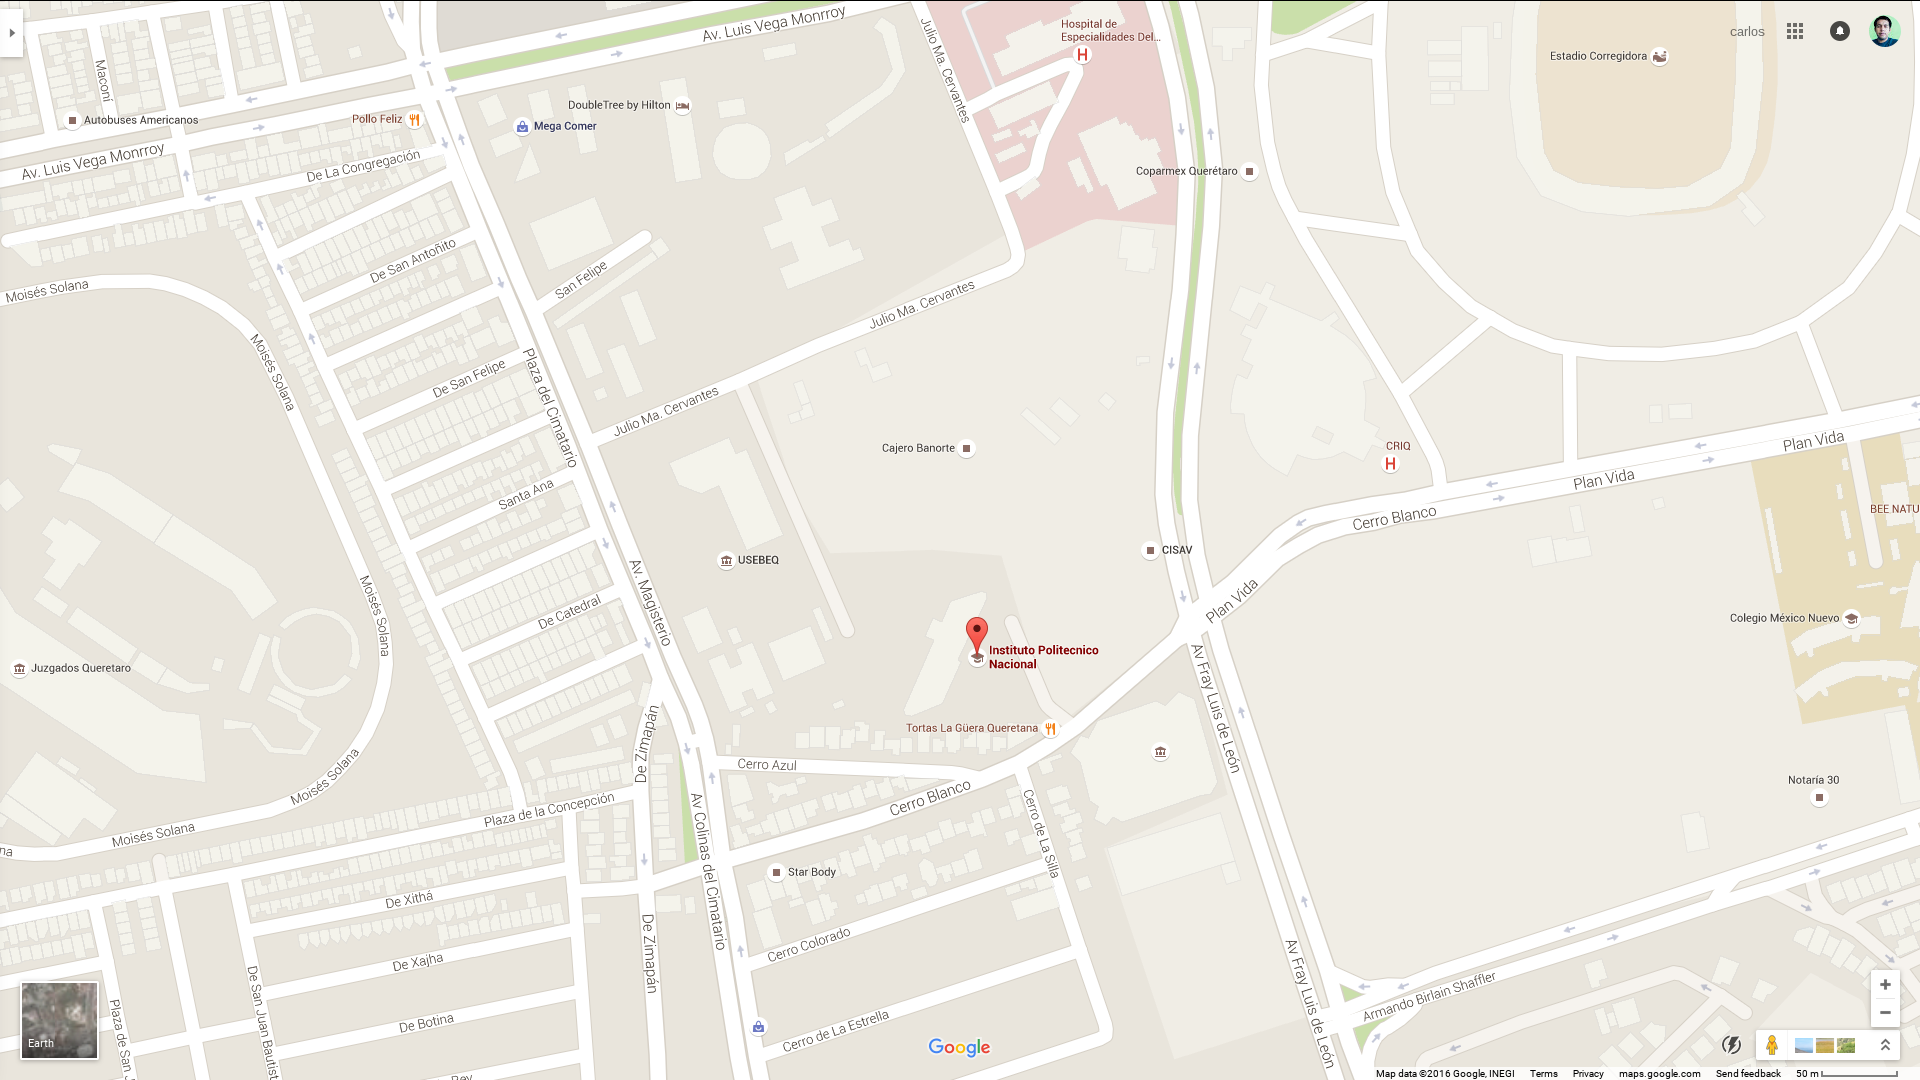
\includegraphics[width=0.9\textwidth]{./imagenes/cicata}
			 \end{center}
		\item[Teléfonos:] 1 (442) 2290804 o 01 (55) 5729 6000 Ext. 81002
		\item[E-Mail:] cicata@ipn.mx 
		\item[Fax:] 5395 4147
	\end{description}
		\subsubsection{Misión}
			Somos un centro de investigación creado por el IPN para fortalecer su impacto a nivel nacional, que atiende
			necesidades de formación de recursos humanos y de desarrollo tecnológico de la región, a través de proyectos
			de investigación que contribuyen al desarrollo social y a la competitividad de los sectores productivo y de
			servicios, con el respaldo de las capacidades del Instituto, con un enfoque multidisciplinario, innovador y
			de excelencia, en un marco de sustentabilidad.
		
		\subsubsection{Visión}
			En el 2025, el CICATA-Querétaro se ve como un centro de vanguardia en la investigación y formación de 
			recursos humanos; referente a nivel latinoamericano; con reconocimiento internacional por sus contribuciones
			de alto impacto y como una de las primeras opciones para alumnos e investigadores, por ser un centro
			innovador, competitivo, líder y emprendedor.
		
		\subsubsection{Valores}
			Hemos identificado un conjunto de valores que nos representan y que permiten cumplir nuestra misión y lograr
			la visión forjada:
			\begin{multicols}{2}
				\begin{itemize}
					\item Calidad
					\item Integridad
					\item Compromiso
					\item Asertividad
					\item Trabajo en equipo
					\item Aprendizaje continuo
				\end{itemize}
			\end{multicols}		
			
		\subsubsection{Objetivo}
			Servir de enlace entre la comunidad científica y los sectores productivos de bienes y servicios, atenderlos
			y ofrecerles soluciones a sus problemas de desarrollo. Para el cumplimiento de este objetivo, CICATA
			Querétaro desarrolla programas de investigación científica, tecnológica e innovación con un enfoque
			interdisciplinario, y asimismo atiende la formación de capital humano de alto nivel, contribuyendo
 			decisivamente al fortalecimiento de la calidad y la competitividad del aparato productivo mexicano.
 		
 		\subsubsection{Estructura Organizativa}
 			\begin{center}
			 	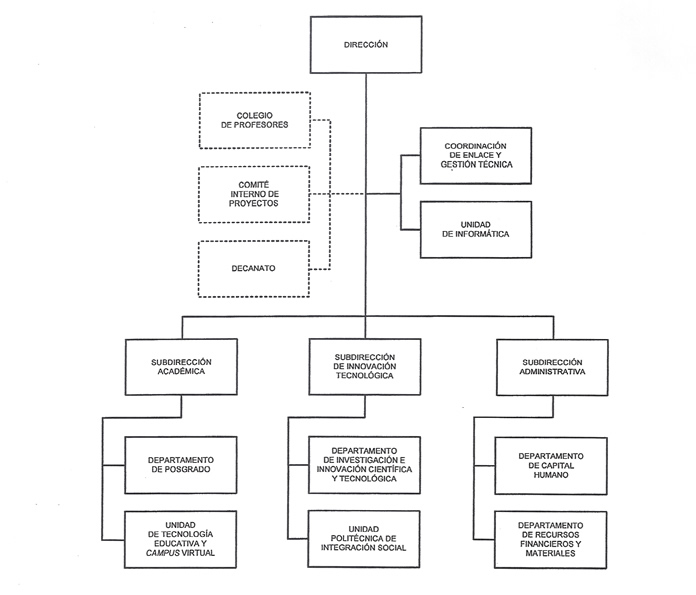
\includegraphics[width=0.9\textwidth]{./imagenes/organigrama}
			 \end{center}
			 
	
	\subsection{Descripción del departamento o área de trabajo}
		 El área de análisis de imágenes puede ser definida como la construcción de algoritmos para la extracción de 
		 información presente en las imágenes. Es un área donde una gran variedad de conceptos fundamentales necesitan 
		 ser desarrollado e importantes aplicaciones pueden crearse. Esta combinación de teoría y práctica es particularmente 
		 atractiva para CICATA Querétaro en virtud de corresponder con su objetivo operativo. El grupo de análisis de imágenes 
		 ha presentado desde sus orígenes resultados muy buenos en el renglón de vinculación y desarrollo tecnológico.  
		 Se han trabajado proyectos de vinculación con empresas e instituciones tales como TAMSA y el IFE, por mencionar algunos. 
		 En la actualidad con un grupo de cuatro investigadores esta tendencia se ha mantenido.  En este momento se estudian 
		 temas de interferometría, colorimetría, industrial, metrología, óptica, análisis de imágenes, procesamiento de imágenes, 
		 reconstrucción tridimensional e interpretación visual de la actividad.

\section{Problemas a resolver}
	\begin{multicols}{2}
	\begin{itemize}
		\item Amplificar áreas de la pantalla donde se enfoque la vista usando la vista.
		\item Detectar y seguir la dirección de la mirada.
		\item Proporcionar una mayor accesibilidad a débiles visuales.
	\end{itemize}
	\end{multicols}
\newpage
\section{Alcances y limitaciones}
	\subsection{Alcances}
		El sistema de seguimiento e identificación de la dirección de la mirada persigue el objetivo de permitir la interacción 
		usuario-maquina usando en el proceso únicamente los ojos y, proporcionar interactividad a esta parte del cuerpo.\\
		
		El uso directo e inmediato de la detección de la dirección de la mirada es el de proporcionar una forma interactiva 
		para magnificar zonas de la pantalla donde se enfoque la mirada en un todo momento.\\
		
		Inicialmente el sistema será desarrollado para funcionar en maquinas con sistema operativo Microsoft Windows.\\
		
	\subsection{Limitaciones}
		Ciertamente el proyecto presenta algunas dificultades técnicas y algunas otras funcionales, entre las cuales encontramos
		las siguiente:\\
		
		Las condiciones no controladas, se esperan condiciones de operación dentro de ciertos parámetros, el rendimiento se puede 
		ver afectado acorde a las condiciones del entorno.\\
		
		La API de magnificación de Microsoft Windows esta solo disponible en para arquitecturas de 32 bits, lo que imposibilita el desarrollo
		del sistema para arquitecturas de 64 bits.\\
	
		
		 

\chapter{FUNDAMENTACIÓN TEÓRICA}
\markboth{FUNDAMENTACIÓN TEÓRICA}{FUNDAMENTACIÓN TEÓRICA} 
\thispagestyle{empty}
\newpage
\section{Ingeniería del software}
	\subsection{Concepto de Software}
		Existen varias definiciones similares aceptadas para software, pero probablemente la más formal sea la siguiente:\\
		
		“Es el conjunto de los programas de cómputo, procedimientos, reglas, documentación y datos asociados que forman parte de las
		operaciones de un sistema de computación” (IEEE Std, 1993).\\
		
		Considerando esta definición, el concepto de software va más allá de los programas de computación en sus distintos estados: 
		código fuente, binario o ejecutable; también su documentación, los datos a procesar e incluso la información de usuario forman
		parte del software: es decir, abarca todo lo intangible, todo lo «no físico» relacionado.\\
		
		El término software fue usado por primera vez en este sentido por John W. Tukey en 1957. En la ingeniería de software y las
		ciencias de la computación, el software es toda la información procesada por los sistemas informáticos: programas y datos.
		
	\subsection{Clasificación del software \label{clasSoft}}
		Si bien la definición anterior de software es, en cierto modo arbitraria, y a veces confusa, a los fines prácticos se puede
		clasificar al software en tres grandes tipos \cite{IngSoft}:
		
	
		\begin{itemize}
			\item \textbf{Software de sistemas:} Su objetivo es desvincular adecuadamente al usuario y al programador de los detalles
			informáticos en particular que se use, aislándolo especialmente del procesamiento referido a las características internas de:
			memoria, discos, puertos y dispositivos de comunicaciones, impresoras, pantallas y teclados. El software de sistema le procura
			al usuario y programador adecuadas interfaces de alto nivel, controlador, herramientas y utilidades que permiten el 
			mantenimiento del sistema global. 
			
			Incluye entre otros:
			\begin{multicols}{2}
				\begin{itemize}
					\item Sistemas Operativos
					\item Controladores de dispositivos
					\item Herramientas de diagnostico
					\item Servidor de utilidades
					\item Herramientas de corrección y optimización.
				\end{itemize}
			\end{multicols}
			
			\item \textbf{Software de programación:} Es el conjunto de herramientas que permiten al programador desarrollar programas
			informáticos, usando diferentes alternativas y lenguajes de programación, de una manera práctica. Incluyen básicamente:
			\begin{multicols}{2}
				\begin{itemize}
					\item Editores de texto
					\item Compiladores
					\item Interpretes
					\item Enlazadores
					\item Depuradores
				\end{itemize}
			\end{multicols}
			\begin{itemize}
				\item Entornos de desarrollo integrado (\textsc{IDE}). Agrupan las anteriores herramientas, usualmente en un entorno
				visual, de forma que el programador no necesite introducir múltiples instrucciones para compilar , interpretar y depurar.
				Cuentan con una interfaz gráfica de usuario \textsc{GUI}.
			\end{itemize}
			
			\item \textbf{Software de aplicacion:} es aquel que permite a los usuarios llevar a cabo una o varias tareas específicas, en
			cualquier campo de actividad susceptible de ser automatizadas o asistido, con especial énfasis en los negocios. Incluye entre
			muchos otros:
			\begin{multicols}{2}
				\begin{itemize}
					\item Control de sistemas.
					\item Automatización industrial
					\item Software educativo
					\item Software empresarial
					\item Base de datos
					\item Telecomunicaciones
					\item Videojuegos
					\item Software medico
					\item Aplicaciones ofimáticas
					\item Software de calculo numérico y simbólico
					\item Diseño asistido (\textsc{CAD})
				\end{itemize}
			\end{multicols}
		\end{itemize}
		
	\subsection{Concepto de la Ingeniería de Software}
		La ingeniería de software es una disciplina de la ingeniería que comprende todos los aspectos de la producción de software desde 
		las etapas iniciales de la especificación del sistema, hasta el mantenimiento de éste después de que se utiliza.
		En esta definición existen dos frases clave:
		\begin{description}
			\item[Disciplina de la ingeniería: ] Los ingenieros hacen que las cosas funcionen. Aplican teorías, métodos y herramientas 	
			donde sean convenientes, pero las utiliza de forma selectiva y siempre tratando de descubrir soluciones a los problemas, aun 
			cuando no existan teorías o métodos aplicables para resolverlos.
			\item[Todos los aspectos de producción de software: ] La ingeniería de software no solo comprende los procesos técnicos del 
			desarrollo de software, sino también actividades tales como la gestión de proyectos de software y el desarrollo de 
			herramientas, métodos y teorías de apoyo a la producción de software.
		\end{description}		 
		en general los ingenieros de software adoptan un enfoque sistemático y organizado en su trabajo, ya que es la forma mas efectiva
		de producir software de calidad \cite{IngSoft} pp.6.
\newpage
\section{Herramientas de desarrollo}
	Como se describe en la sección \ref{clasSoft} hay diferentes clases y tipos de software, entre los que se encuentran las herramientas
	de 	desarrollo o software de desarrollo, así como software de aplicación, en este proyecto se han usado variedad de ellas, de las 
	cuales se da una descripción a continuación:
	\subsection*{Software de desarrollo}	
	\subsection{Visual Studio Community 2015 \label{VS}}
		\textsc{Visual Studio Community 2015} [\ref{i_vs}] es un entorno de desarrollo integrado creado y distribuido por \textsc{Microsoft}, 
		para el sistema operativo de la misma.
		Soporta una gran variedad de lenguajes de programación tales como, \textsc{ C++, C\#, Visual Basic, .NET, F\#, Java, Python, 
		Ruby, PHP}, al igual que entornos de desarrollo web como \textsc{ASP.NET MVC, Django, etc.,} a lo cual sumarle las nuevas
		capacidades online bajo Windows Azure en forma del editor Monaco.
		Esta version en particular tiene la particularidad de ser gratuita e incluir todas las características de la versión 
		\textsc{Express}, enfocada en desarrolladores individuales, proyectos de código abierto, investigación académica, educación
		y pequeños equipos  de profesionales.
		
	\subsection{Qt Creator \label{qt}}
		\textsc{Qt Creator} [\ref{i_crator}] es un IDE (entorno de desarrollo integrado) multiplataforma que se ajusta a las necesidades de los 
		desarrolladores Qt. 
		Este es parte de Qt Project \footnote{\textit{\scriptsize \href{http://www.qt.io/}{Qt Project}}}.
		
		Qt Creator se centra en proporcionar características que ayudan a los nuevos usuarios de Qt a aprender y comenzar a desarrollar
		rápidamente, también aumenta la productividad de los desarrolladores con experiencia en Qt.
		\begin{multicols}{2}
		\begin{itemize}
			\item Editor de código con soporte para C+, QML y ECMAscript
			\item Herramientas para la rapida navegacion del codigo
	    	\item Resaltado de sintaxis y auto-completado de código
			\item Control estático de código y estilo a medida que se escribe
		    \item Soporte para refactoring de código
	    	\item Ayuda sensitiva al contexto
		    \item Plegado de código (code folding)
	    	\item Paréntesis coincidentes y modos de selección
		\end{itemize}
		\end{multicols}
	
	\subsection{PyCharm \label{pych}}
		\textsc{Pycharm} [\ref{i_pycharm}] es un entorno integrado de desarrollo (\textsc{IDE}) usado para la programacion en \textsc{Python} 
		(\ref{python}). 
		Provee herramientas de análisis de código, depurador gráfico, pruebas unitarias, integración con sistemas de control de versiones
		y soporte para el desarrollo con \textsc{Django}.\\
		Desarrollado por la compañía \href{https://en.wikipedia.org/wiki/JetBrains}{JetBrains}
		\footnote{\scriptsize JetBrains: https://en.wikipedia.org/wiki/JetBrains}.\\
		
		Es multi-plataforma, funcionando en Windows, Mac OS X y Linux, cuenta con una version profesional liberada bajo licencia 
		propietaria y con una versión comunitaria bajo los términos de \href {https://en.wikipedia.org/wiki/Apache_License}{Apache Licence}
		\footnote{\scriptsize Apache: https://en.wikipedia.org/wiki/Apache\_License}, aunque esta última cuenta con algunas limitaciones.\\
		
		Entre sus características mas destables se encuentran las siguientes:
		\begin{multicols}{2}
		\begin{itemize}
			\item Asistencia en el análisis de código
			\item Auto-completado de código
			\item Errores de sintaxis
			\item Resaltado de lineas
			\item Vistas de navegación
			\item Vistas de estructuras
			\item Integración con Python Debugguer.
			\item Integración con CVS.
		\end{itemize}
		\end{multicols}
		\begin{figure}[hbt]
			\centering
			\subfigure[PyCharm]{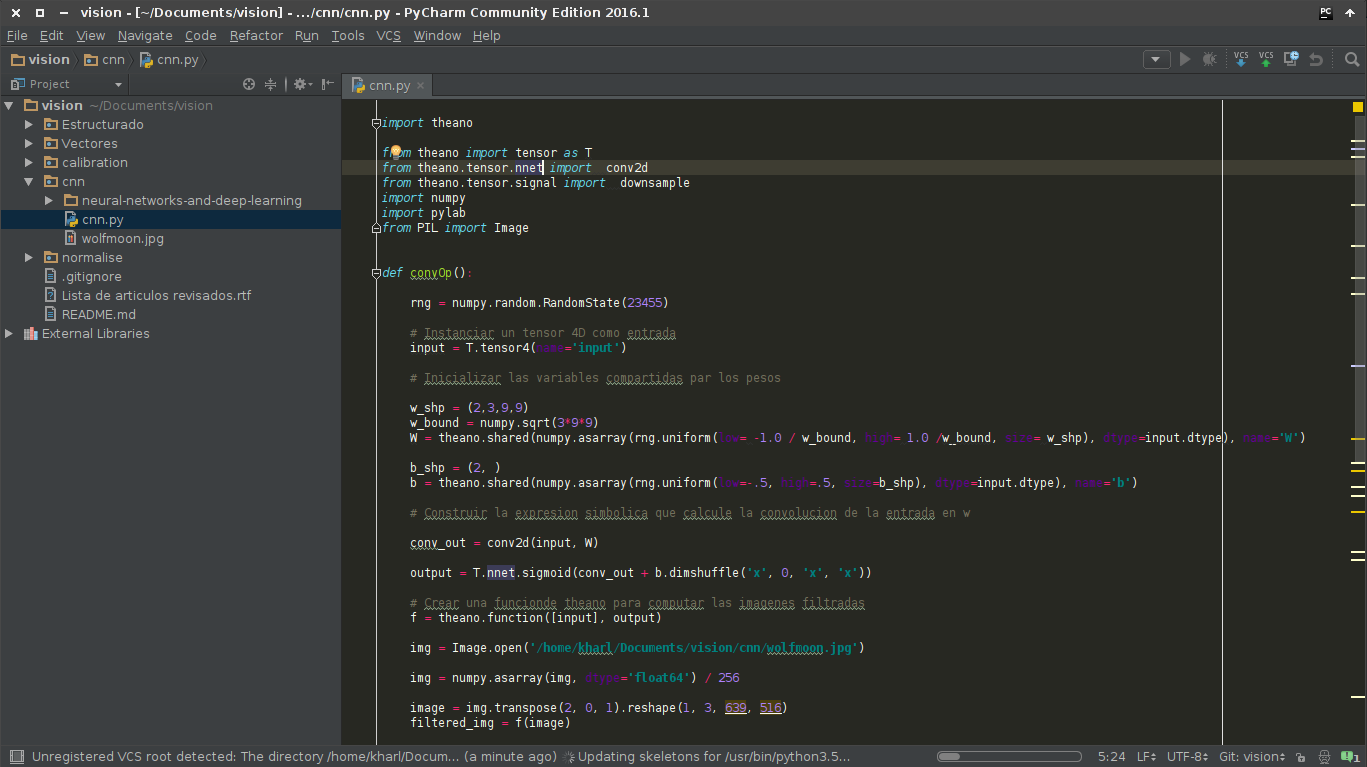
\includegraphics[width=110mm]{pycharm.png} \label{i_pycharm}}
			\subfigure[Qt Creator]{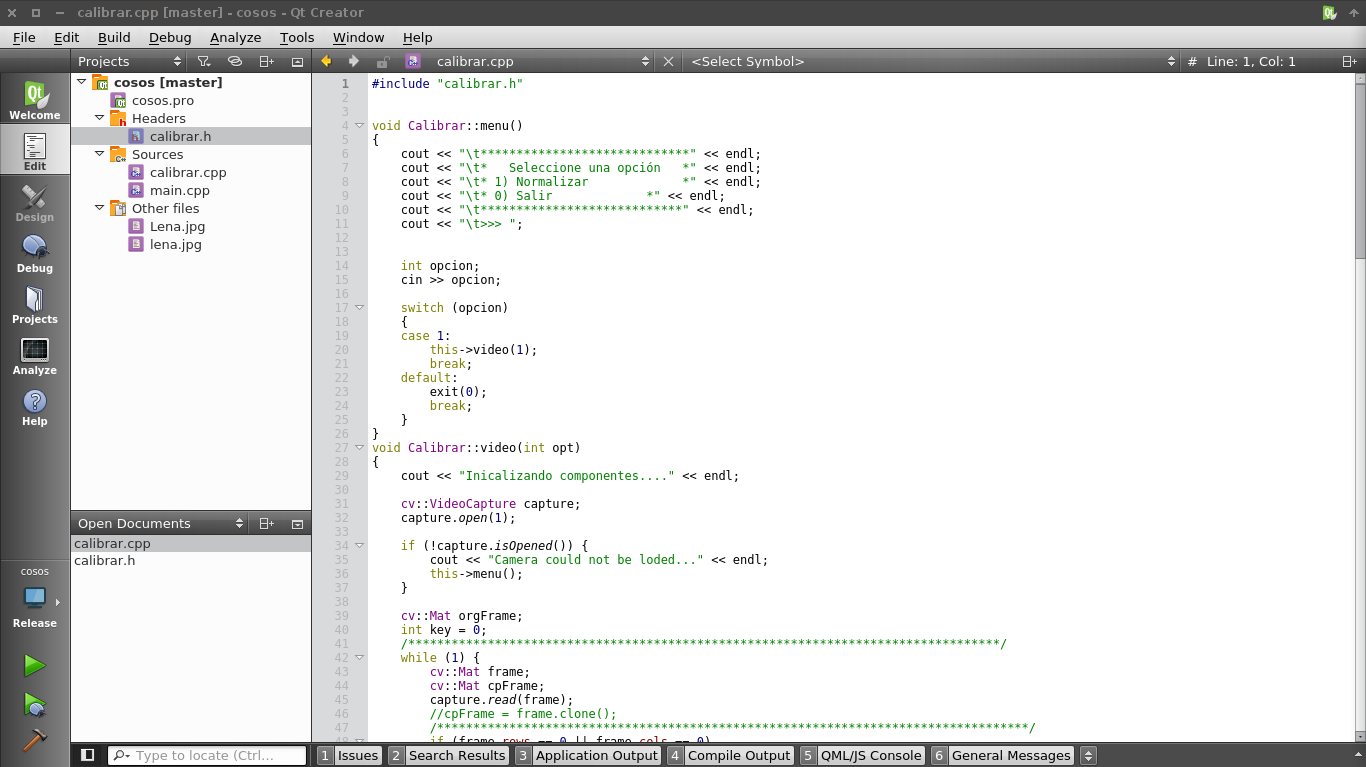
\includegraphics[width=110mm]{qt_creator.png} \label{i_crator}}
			\subfigure[Visual Studio]{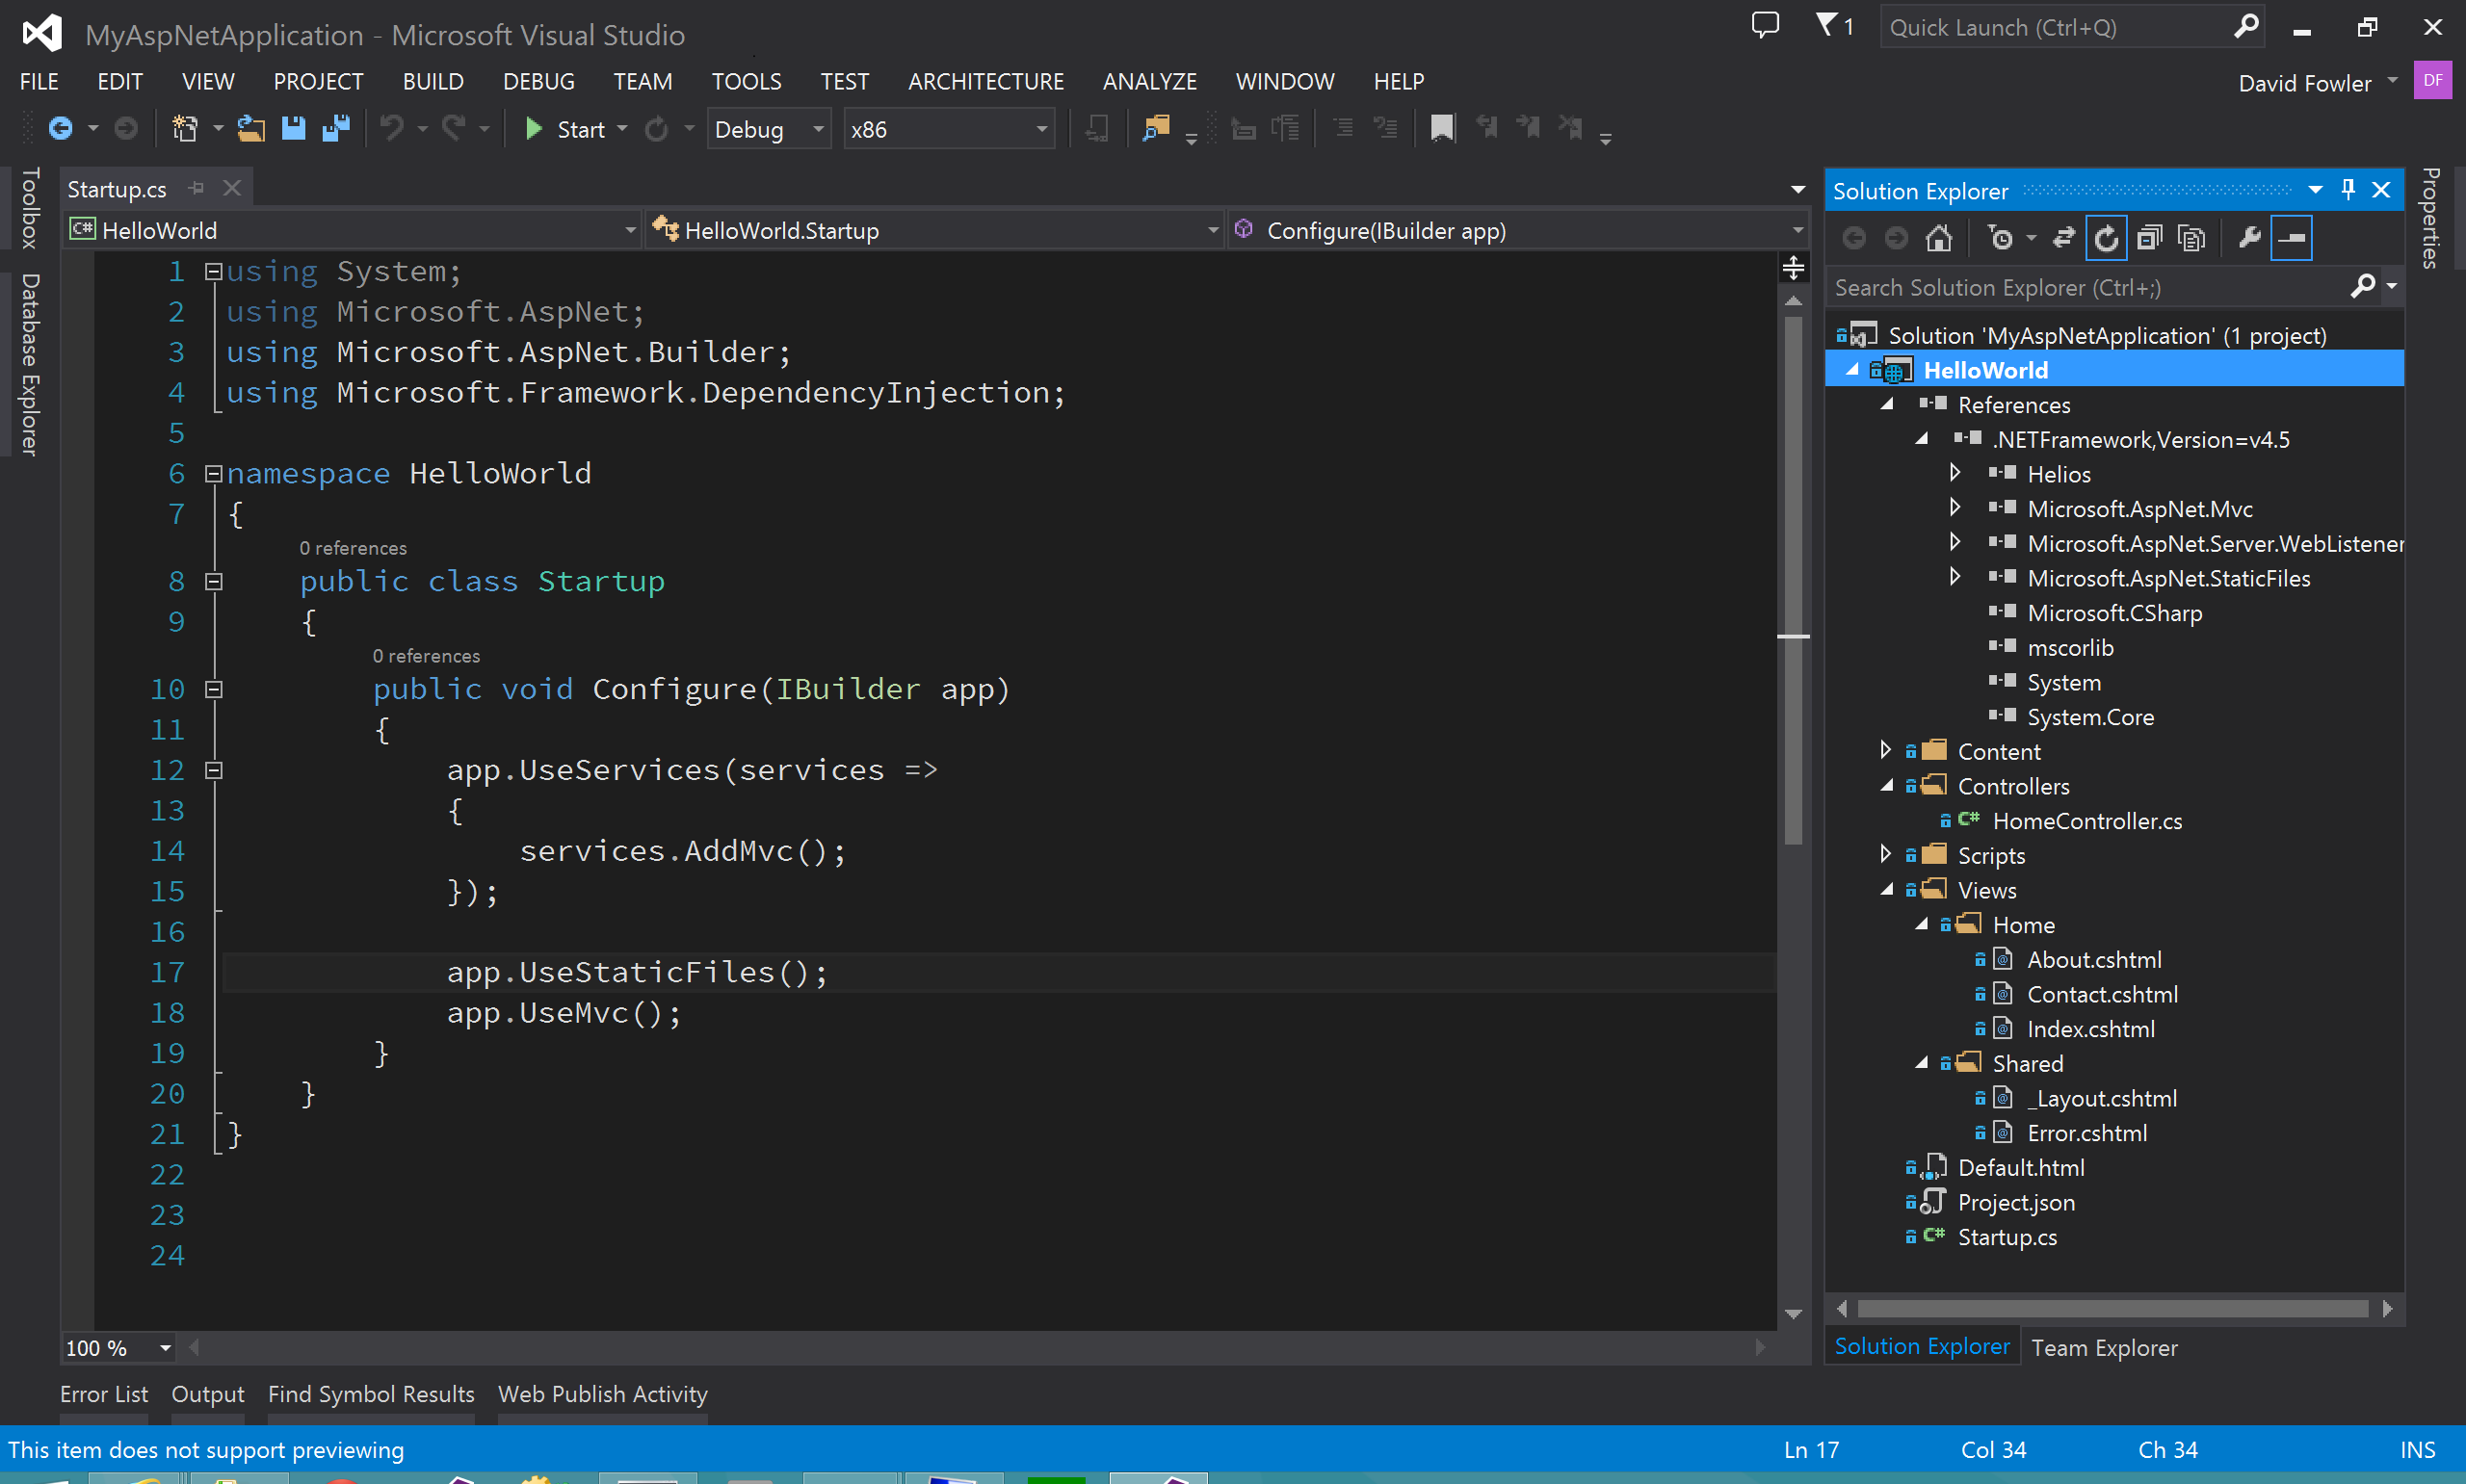
\includegraphics[width=110mm]{vs.png} \label{i_vs}}			
			\caption{Herramientas de desarrollo. \label{f-lenete-uml}}
		\end{figure}	
		\begin{figure}[hbt]
			\centering
			\subfigure[Sublime-Text]{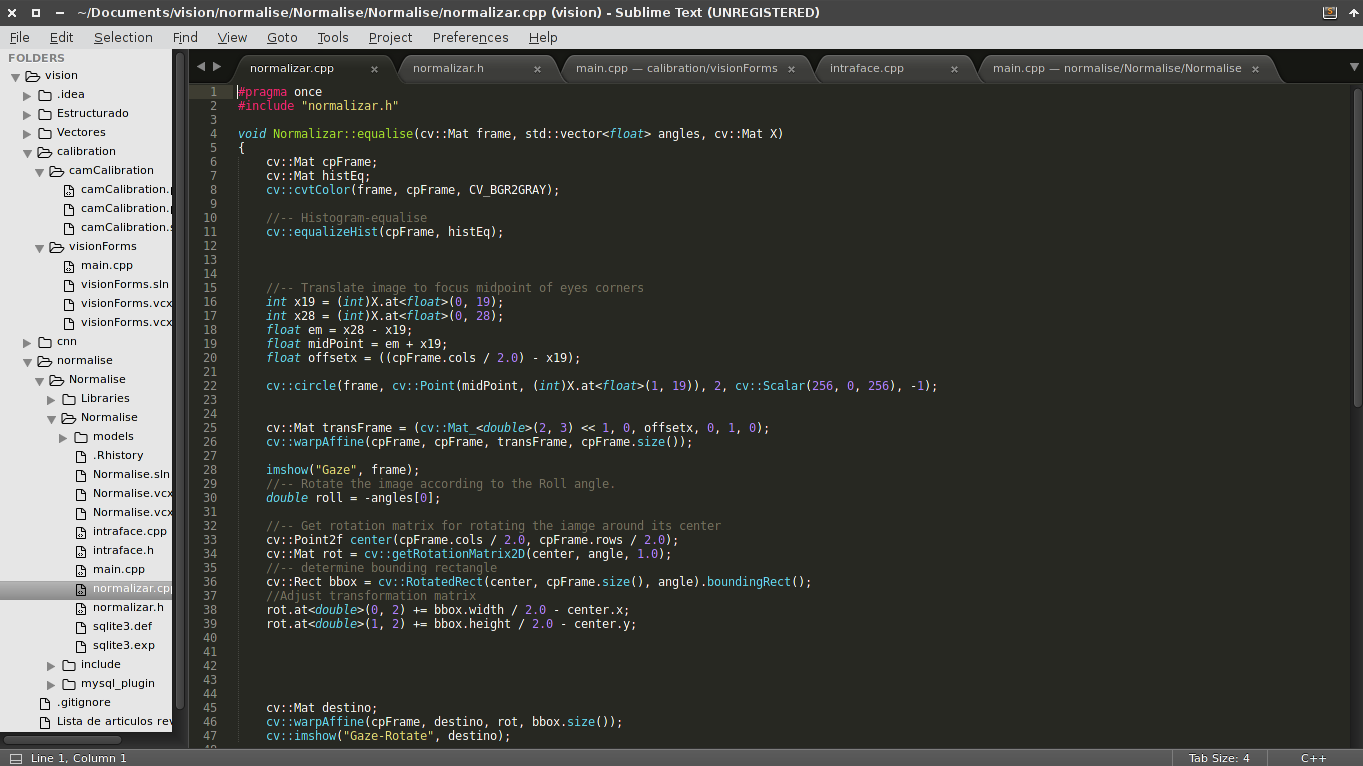
\includegraphics[width=110mm]{subl3.png} \label{i_sublime}}
			\subfigure[RStudio]{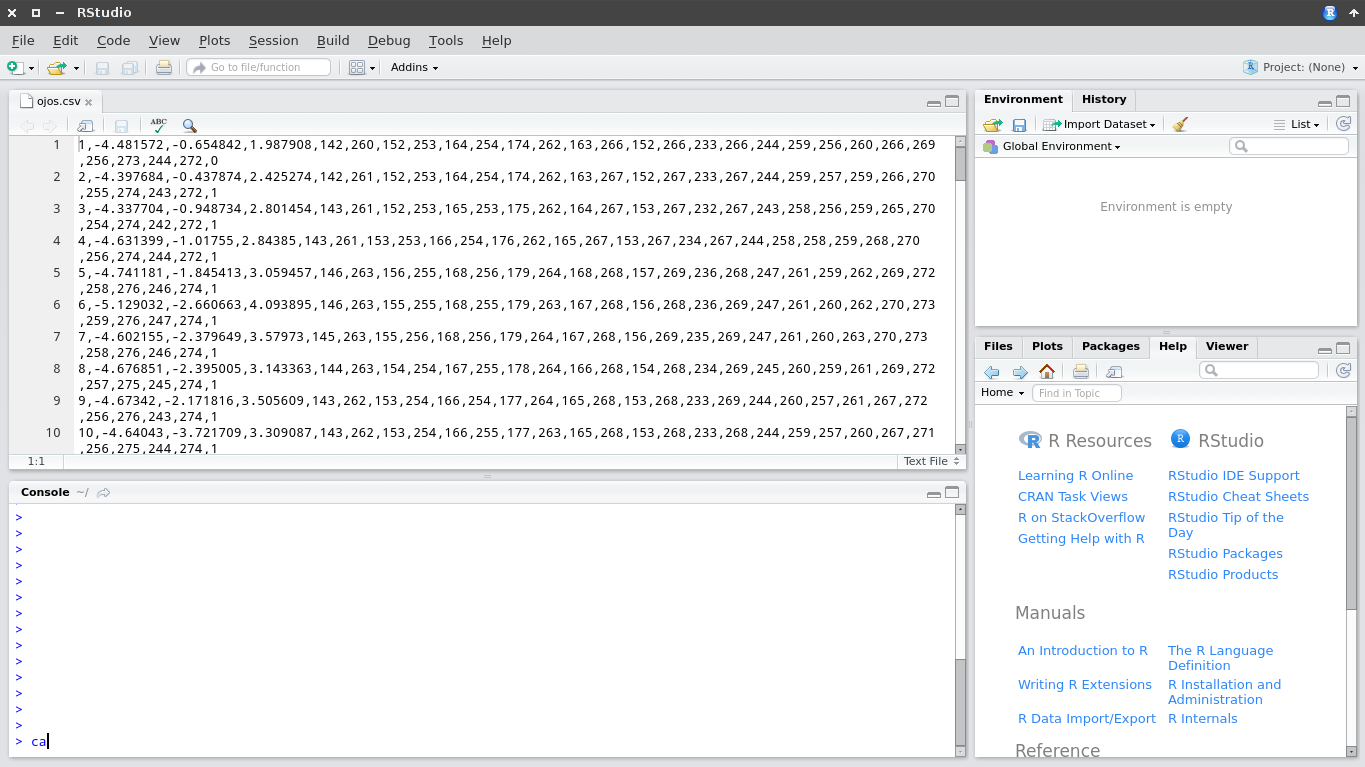
\includegraphics[width=110mm]{rstudio.png} \label{i_rstudio}}
			\subfigure[CMake]{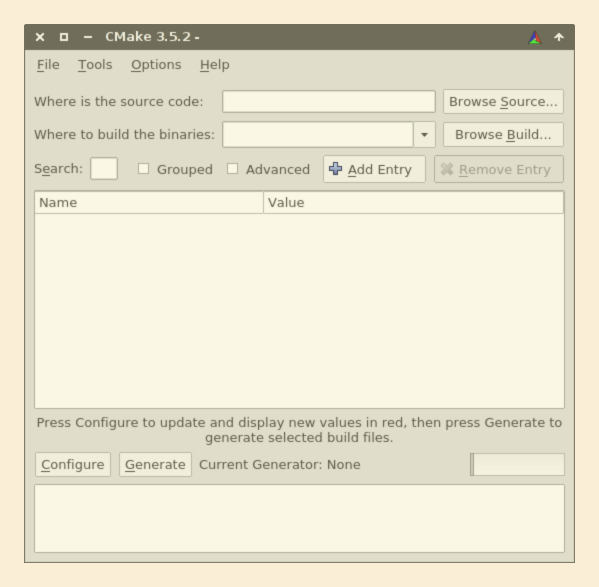
\includegraphics[width=80mm]{cmake.png} \label{i_cmake}}
			\caption{Herramientas de desarrollo. \label{f-lenete-uml}}
		\end{figure}	
	\subsection{Sublime-Text \label{subl}}
		Sublime Text [\ref{i_sublime}] es un editor de texto y editor de código fuente está escrito en C++ y Python para los plugins. Desarrollado
		originalmente como una extensión de \texttt{Vim}, con el tiempo fue creando una identidad propia, por esto aún conserva un modo 
		de edición tipo vi llamado Vintage mode.\\
		
		Características:
		\begin{multicols}{2}
			\begin{itemize}
				 \item Minimapa. consiste en una previsualización de la estructura del código
				 \item Multi selección: Hace una selección múltiple de un término por diferentes partes del archivo.
				 \item Multi cursor: Crea cursores con los que podemos escribir texto de forma arbitraria en diferentes posiciones del
				 	   archivo.
				 \item Multi layout: Trae siete configuraciones de plantilla podemos elegir editar en una sola ventana o hacer una división
				 \item Soporte nativo para infinidad de lenguajes: Soporta de forma nativa 43 lenguajes de programación y texto plano.
				 \item Remarcado de sintaxis: El remarcado de sintaxis es completamente configurable a través de archivos de configuración 
				 	   del usuario.
				 \item Búsqueda dinámica: Se puede hacer búsqueda de expresiones regulares o por archivos, proyectos, directorios, una 
				 	   conjunción de ellos o todo a la vez.
				 \item Keybindings: Todas las teclas pueden ser sobrescritas a nuestro gusto.
				 \item Etc.
			\end{itemize}
		\end{multicols}
		
		Se puede descargar desde el sitio web \href{https://www.sublimetext.com/}{Sublime-Text} 
		\footnote{\scriptsize Subl-Text: https://www.sublimetext.com/}
		y evaluar de forma gratuita. Sin embargo no es software libre o de código abiertoy se debe obtener una licencia 	para su uso
		continuado, aunque la versión de evaluación es plenamente funcional y no tiene fecha de caducidad.
				
		
		
	\subsection{Rstudio \label{RS}}
		RStudio [\ref{i_rstudio}] es un entorno de desarrollo integrado (\textsc{IDE}) para R (\ref{r}).\
		Esta disponible de forma libres y en edición comercial, se ejecuta en entornos multiplataforma (Windows, Mac OS X y Linux) o
		sobre navegadores web conectados a \textsc{RStudio Server o RStudio Server Pro (Debian/Ubuntu, RedHat/CentOS y SUSE Linux)}.\\
		
		RStudio tiene la misión de proporcionar el entorno informático estadístico R. Permite un análisis y desarrollo para que 
		cualquiera pueda analizar los datos con R.
		
		Entre sus características se encuentran la siguientes:
		\begin{multicols}{2}
			\begin{itemize}
				\item Consola integrada
				\item Resaltado de sintaxis
				\item Ejecución directa de código R.
				\item Herramientas para gráficos
				\item Historial
				\item Depurador interactivo
				\item Fácil administración de espacios de trabajo.
				\item Ayuda y documentación integrada
				\item Edición con Sweave y R Markdown
			\end{itemize}
		\end{multicols} 
		Esta disponible desde la web oficial del proyecto \href{https://www.rstudio.com/}{RStudio} 
		\footnote{\scriptsize RStudio: https://www.rstudio.com/} en sus dos versiones.\\
		
		
	
	\subsection{CMake \label{CM}}
		\textsc{CMake} [\ref{i_cmake}] es una herramienta multiplataforma de generación o automatización de código. El nombre es una abreviatura para 
		\textit{'cross platform make' (make multiplataforma)}; más allá del uso de \textit{'make'} en el nombre, CMake es una suite separada 
		y de más alto nivel que el sistema \texttt{make} común de Unix, siendo similar a las autotools.
		
		CMake es una familia de herramientas diseñada para construir, probar y empaquetar software. CMake se utiliza para controlar el
		proceso de compilación del software usando ficheros de configuración sencillos e independientes de la plataforma. 
		
		Desarrollado por \textit{Andy Cedilnik, Bill Hoffman, Brad King, Ken Martin, Alexander Neundorf} se puede acceder a la ultima 
		version estable en \href{www.cmake.org}{CMake} \footnote{\scriptsize CMake: www.cmake.org}.\\
		
		Entre las principales funcionalidad se encuentran las siguientes:
		\begin{multicols}{2}
			\begin{itemize}
				\item Ficheros de configuración escritos en un lenguaje de scripting específico para CMake
				\item Análisis automático de dependencias para C, C++, Fortran, y Java
				\item Soporte para SWIG, Qt, FLTK, a través del lenguaje de scripting de CMake
				\item Soporte para varias versiones de Microsoft Visual Studio, incluyendo la 6, 7, 7.1, 8.0, 9.0 y 10.0
				\item Detección de cambios en ficheros usando timestamps tradicionales
				\item Soporte para builds paralelos
				\item Compilador cruzado
				\item Soporte para builds multiplataforma
				\item Integrado con \textsc{DART (software), CDash, CTest y CPack}, una colección de herramientas para prueba y liberación
				 de software
			\end{itemize}
		\end{multicols}
		
	\subsection*{Software de aplicación}
	
	\subsection{Sistema de control de versiones Git \label{git}}
		Git es un software de control de versiones diseñado por \textit{Linus Torvalds}, pensando en la eficiencia y la confiabilidad del
		mantenimiento de versiones de aplicaciones cuando éstas tienen un gran número de archivos de código fuente. Al principio, Git se
		pensó como un motor de bajo nivel sobre el cual otros pudieran escribir la interfaz de usuario o front end como Cogito o StGIT. 
		
		Sin embargo, Git se ha convertido desde entonces en un sistema de control de versiones con funcionalidad plena. Hay algunos
		proyectos de mucha relevancia que usan Git, en particular, el grupo de programación del núcleo Linux.
		
		Entre las características más relevantes se encuentran:
		\begin{multicols}{2}
			\begin{itemize}
				\item Fuerte apoyo al desarrollo no lineal, por ende rapidez en la gestión de ramas y mezclado de diferentes versiones. 
				\item Gestión distribuida, Git le da a cada programador una copia local del historial del desarrollo entero, y los 
				cambios se propagan entre los repositorios locales. 
				\item Los almacenes de información pueden publicarse por HTTP, FTP, rsync o mediante un protocolo nativo, ya sea a través 
				de una conexión TCP/IP simple o a través de cifrado SSH.
				\item Gestión eficiente de proyectos grandes, dada la rapidez de gestión de diferencias entre archivos.
			\end{itemize}
		\end{multicols}
		
		La documentación completa, tutoriales de uso y medios de instalación se pueden encontrar en la pagina oficial de 
		\href{https://git-scm.com/}{Git} \footnote{\scriptsize Git: https://git-scm.com/}
	
		
	\subsection{MariaDB \label{maria}}
		\textsc{MariaDB} es un sistema de gestión de bases de datos derivado de \textsc{MySQL} con licencia \textsc{GPL}. 
		Está desarrollado por \textit{Michael (Monty) Widenius (fundador de MySQL)} y la comunidad de desarrolladores de software 
		libre. 
		
		Introduce dos motores de almacenamiento nuevos, uno llamado Aria -que reemplaza con ventajas a \textsc{MyISAM}- y otro
		lamado \textsc{XtraDB} -en sustitución de \textsc{InnoDB}. Tiene una alta compatibilidad con MySQL ya que posee las mismas
		órdenes, interfaces, APIs y bibliotecas, siendo su objetivo poder cambiar un servidor por otro directamente. 
		Este \textsc{SGBD} surge a raíz de la compra de \textit{Sun Microsystems}.
		
		MariaDB es un fork directo de MySQL que asegura, permanecerá una versión de este producto con licencia GPL. 
		La ultima versión estable se puede encontrar en la web oficial del proyecto \href{https://mariadb.org/}{MariaDB} 
		\footnote{\scriptsize MariaDB: https://mariadb.org/}.
		
	\subsection{SQLite}
		\textsc{SQLite} es un sistema de gestión de bases de datos relacional compatible con \textsc{ACID}, contenida en una
		relativamente pequeña (~275 kiB) biblioteca escrita en C. SQLite es un proyecto de dominio público creado por 
		\textit{D. Richard Hipp}.
		
		A diferencia de los sistema de gestión de bases de datos cliente-servidor, el motor de SQLite no es un proceso independiente 
		con el que el programa principal se comunica. En lugar de eso, la biblioteca SQLite se enlaza con el programa pasando a ser
		parte integral del mismo. 
		
		El programa utiliza la funcionalidad de SQLite a través de llamadas simples a subrutinas y funciones. Esto reduce la latencia 
		en el acceso a la base de datos, debido a que las llamadas a funciones son más eficientes que la comunicación entre procesos. 
		El conjunto de la base de datos (definiciones, tablas, índices, y los propios datos), son guardados como un sólo fichero
		estándar en la máquina cliente. 
		Este diseño simple se logra bloqueando todo el fichero de base de datos al principio de cada transacción.
		
		En su versión 3, SQLite permite bases de datos de hasta \textsc{2 Terabytes} de tamaño, y también permite la inclusión de campos
		tipo \textsc{BLOB}.
		
	\subsection*{Librerías}	
	
	\subsection{OpenCV \label{cv}}
			
		
		\textsc{OpenCV} es una biblioteca libre de visión artificial originalmente desarrollada por \textsc{Intel}. 
		Desde que apareció su primera versión alfa en el mes de enero de 1999, se ha utilizado en infinidad de aplicaciones. 
		Desde sistemas de seguridad con detección de movimiento, hasta aplicaciones de control de procesos donde se requiere
		reconocimiento de objetos. Esto se debe a que su publicación se da bajo licencia \textsc{BSD}, que permite que sea usada
		libremente para propósitos comerciales y de investigación con las condiciones en ella expresadas.
		
		OpenCV es multiplataforma, existiendo versiones para \textsc{GNU/Linux, Mac OS X y Windows}. Contiene más de 500 funciones 
		que abarcan una gran gama de áreas en el proceso de visión, como reconocimiento de objetos (reconocimiento facial), 
		calibración de cámaras, visión estérea y visión robótica.
		
		El proyecto pretende proporcionar un entorno de desarrollo fácil de utilizar y altamente eficiente. Esto se ha logrado
		realizando su programación en código C y C++ optimizados, aprovechando además las capacidades que proveen los procesadores
		multinúcleo. OpenCV puede además utilizar el sistema de primitivas de rendimiento integradas de Intel, un conjunto de 
		rutinas de bajo nivel específicas para procesadores Intel \textsc{(IPP)}.
		
		
	\subsection{IntraFace \label{intraface}}
		IntraFace es una librería que incluye algoritmos para análisis de patrones faciales, se comenzó a desarrollar en 2010 en la
		universidad \textsc{Carnigie Mellon \& University of Pittsburgh}, actualmente la ultima version de la misma es la 1.0, soportada 
		por Human Sensing Laboratory.\\
		Para este proyecto se usa una version anterior de la misma, provista para fines educativos y/o investigación sin fines de lucro.

	
		
\newpage		
	
\section{Lenguajes de programación}
	
	Un lenguaje de programación es un lenguaje formal diseñado para realizar procesos que pueden ser llevados a cabo por máquinas como las computadoras.
	Pueden usarse para crear programas que controlen el comportamiento físico y lógico de una máquina, para expresar algoritmos con precisión, o como 
	modo de comunicación humana.\\
	Está formado por un conjunto de símbolos, reglas sintácticas y semánticas que definen su estructura y el significado de sus elementos y expresiones. 
	al proceso por el cual se escribe, se prueba, se depura, se compila (de ser necesario) y se mantiene el código fuente de un programa informático se 
	le llama programación.\\
	
	También la palabra programación se define como el proceso de creación de un programa de computadora, mediante la aplicación de procedimientos 
	lógicos, a través de los siguientes pasos:
	\begin{multicols}{2}	
		\begin{itemize}
			\item El desarrollo lógico del programa para resolver un problema en particular.
			\item Escritura de la lógica del programa empleando un lenguaje de programación específico \textit{(codificación del programa)}
			\item Ensamblaje o compilación del programa hasta convertirlo en lenguaje de máquina.
			\item Prueba y depuración del programa.
			\item Desarrollo de la documentación.
		\end{itemize}
	\end{multicols}
	
	Existen multitud lenguajes disponibles en la actualidad, en este proyecto y dadas las características del mismo, los lenguajes que más se 
	adaptan a estas son los siguientes:
	\begin{multicols}{3}	
		\begin{itemize}
			\item \texttt{C++}
			\item \texttt{Python}
			\item \texttt{R}		
		\end{itemize}
	\end{multicols}
	
	\subsection{C++}
		\textsc{C++} es un lenguaje de programación diseñado a mediados de los años 1980 por \textit{Bjarne Stroustrup}. La intención 
		de su creación fue el extender al lenguaje de programación \textsc{C}, agregando mecanismos que permitieran la manipulación de
		objetos. En ese sentido, desde el punto de vista de los lenguajes orientados a objetos, el C++ es un lenguaje híbrido, por un lado 
		es un lenguaje que sigue muy ligado a hardware subyacente, manteniendo una considerable potencia para la programación a bajo nivel, 
		pero se le han añadido elementos que le permiten un estilo de programación de alto nivel de abstracción.
		
		La definición oficial nos dice que C++ es un lenguaje de propósito general basado en C, al que se le han añadido nuevos tipos de 
		datos, plantillas, clases, mecanismos de acepciones, espacio de nombres (STD), funciones inline, sobrecarga de operadores, 
		referencias, manejo de memoria persistente y algunas utilidades adicionales en la librería estándar de C++.
		
		\subsubsection{Historia}
			El comité para el estándar ANSI C fue formado en 1983 con el objetivo de crear un lenguaje uniforme a partir del C original,
			desarrollado por \textit{Kernighan y Ritchie} en 1972, en la AT\&T. Hasta entonces el estándar lo marcaba el libro escrito en
			1978 por estos dos autores. 
			El lenguaje C++ se comenzó a desarrollar en 1980. Su autor fue Bjarne Stroustrup, también de la AT\&T. 
			Al comienzo era una extensión del lenguaje C que fue denominada \textit{C with classes}. Este nuevo lenguaje comenzó a ser
			utilizado fuera de la AT\&T en 1983. El nombre C++ es también de ese año, y hace referencia al carácter del operador incremento
			de C (++). Ante la gran difusión y éxito que iba obteniendo en el mundo de los programadores, la AT\&T comenzó a estandarizarlo
			internamente en 1987. En 1989 se formó un comité ANSI (seguido algún tiempo después por un comité ISO) para estandarizarlo a
			nivel americano e internacional.
			
		 \subsubsection{Características}
		 	Antes, mencionar que tanto C como C++ son lenguajes compilados, y no interpretados. Esta diferencia es muy importante, ya que
		 	afecta mucho a muchos aspectos relacionados con la ejecución del programa.\\
		 	
		 	Como lenguaje de programación orientado a objetos  se basa en una filosofía completamente diferente a la se su predecesor, exige 
		 	el cambio completo de paradigma al programador, las propias características de la Programación Orientada a Objetos de C++ son 
		 	la causa principal de ello.
		 
		
		
	\subsection{Python \label{python}}
		Python es un lenguaje de programación creado por Guido van Rossum a principios de los años 90 cuyo nombre está inspirado en el grupo
		de cómicos ingleses \textit{Monty Python}. Es un lenguaje similar a Perl, pero con una sintaxis muy limpia y que favorece un código 
		legible \cite{python}.
		
		Se trata de un lenguaje interpretado o de script, con tipado dinámico, fuertemente tipado, multiplataforma y orientado a objetos.\\
		
		El intérprete de Python está disponible en multitud de plataformas (\textsc{UNIX, Solaris, Linux, DOS, Windows, OS/2, Mac OS}, etc.)
		por lo que si no utilizamos librerías específicas de cada plataforma nuestro programa podrá correr en todos estos sistemas sin
		grandes cambios.\\
		Python es un lenguaje que todo el mundo debería conocer. Su sintaxis simple, clara y sencilla; el tipado dinámico, el gestor de
		memoria, la gran cantidad de librerías disponibles y la potencia del lenguaje, entre otros, hacen que desarrollar una aplicación en
		Python sea sencillo, muy rápido y, lo que es más importante, divertido.\\		
		
		Python no es adecuado sin embargo para la programación de bajo nivel o para aplicaciones en las que el rendimiento sea crítico.\\
		Algunos casos de éxito en el uso de Python son Google, Yahoo, la NASA, Industrias Ligh \& Magic, y todas las distribuciones Linux, 
		en  las que Python cada vez representa un tanto por ciento mayor de los programas disponibles.
		
		\subsubsection{Instalacion de Python}
			Existen varias implementaciones distintas de Python: CPython, Jython, IronPython, PyPy, etc	
			
			CPython es la más utilizada, la más rápida y la más madura. Cuando la gente habla de Python normalmente se refiere a esta
			implementación. 
			En este caso tanto el intérprete como los módulos están escritos en C.\\
			
			Jython es la implementación en Java de Python, mientras que IronPython es su contrapartida en C\# (.NET). Su interés estriva en 
			que utilizando estas implementaciones se pueden utilizar todas las librerías disponibles para los programadores de Java y .NET.

			PyPy, por último, como habréis adivinado por el nombre, se trata de una implementación en Python de Python.
			
			CPython está instalado por defecto en la mayor parte de las distribuciones Linux y en las últimas versiones de Mac OS. Para
			comprobar si está instalado abre una terminal y escribe \texttt{python}. Si está instalado se iniciará la consola interactiva 
			de Python y obtendremos parecido a lo siguiente:
			
			\begin{minipage}[t]{0.3\textwidth}
			\scriptsize			
				\begin{verbatim}

					Python 3.5.1 (default, Mar  3 2016, 09:29:07)
					[GCC 5.3.0] on linux
					Type "help", "copyright", "credits" or "license" for more information.
					>>> |
				\end{verbatim}			
			\end{minipage}
			\\
			si no te muestra algo parecido no te preocupes, instalar Python es muy sencillo. Puedes descargar la versión correspondiente a
			tu sistema operativo desde la web de \href{https://www.python.org/}{Python} 
			\footnote{\scriptsize Python: \href{https://www.python.org/}{https://www.python.org/}.}
			
		\subsubsection{Herramientas básicas}
			Existen dos formas de ejecutar código Python. Podemos escribir líneas de código en el intérprete y obtener una respuesta del
			intérprete para cada línea (sesión interactiva) o bien podemos escribir el código de un programa en un archivo de texto y
			ejecutarlo.
			
			Para el trabajo del proyecto se uso PyCharm (\ref{pych}) como IDE de desarrollo, anque en algunas ocaciones se uso editor de
			texto, \textsc{Sublime-text} (\ref{subl}) , para la edición rápida.

	\subsection{R \label{r}}
		\subsubsection{¿Qué es R?}
			Comenzaremos diciendoq ue \textsf{R}	es un lenguaje de programación interpretado, de distribucion libre, bajo Licencia GNU,
			y se mantiene en un ambiente para el computo estadistico y gráfico. Este \textit{software} corre en distintas plataformas 
			\textsc{Linux, Mac OS X, Windows} e incluso en \textsf{PlayStation 3}. El termino ambiente pretende caracterizalo como un sistema 
			totalmente planificado y coherente, en lugar de una cumulación gradual de herramientas muy especificas y poco flexibles,
			como suele ser con otro software de análisis de datos. El hecho que R sea un lenguaje y un sistema, es por que forma parte de 
			la filosofía de creación.
			
			Por ello en ves de pensar en R como un sistema estadístico es preferible verlo como un ambiente en el que se aplica técnicas
			estadísticas. Por ejemplo, en este proyecto nos inclinaremos hacia el lado de la programación \textit{(lenguaje)} más que tocar
			los aspectos estadísticos.
			
			\subsubsection{Historia}
			R fue creado en 1992 en Nueva Zelanda por Ross Ihaka y Robert Gentleman (Ihaka [1998]). La intención inicial con R, era hacer 
			un lenguaje didáctico, para ser utilizado en el curso de Introducción a la Estadística de la Universidad de Nueva Zelanda.\\
			Para ello decidieron adoptar las sintaxis similar al lenguaje \textsf{S}, pero la semántica, que aparentemente es parecida a S,
			en realidad es sensiblemente diferente, sobre todo en los detalles un poco más profundos de la programación.
			A modo de broma Ross y Robert, comenzaron a llamar \textsf{R} al lenguaje que implementaron, por las iniciales de sus nombres, 
			y desde entonces así se le conoce en la muy extendida comunidad amante de dicho lenguaje.
		
	
		
\newpage
\section{Metodologías de desarrollo de software}
	
	\subsection{Metodología de desarrollo extremo \label{XP}}
		La programación extrema se basa en una serie de reglas y principios que se han ido gestando a lo largo de toda la historia de la 
		ingeniería del software. Usadas conjuntamente proporcionan una nueva metodología de desarrollo software que se puede englobar dentro
		de las metodologías ligeras, que son aquéllas en la que se da 	prioridad a las tareas que dan resultados directos y que reducen la
		burocracia que hay alrededor tanto como sea posible (pero no más).
		La programación extrema, dentro de las metodologías ágiles, se puede clasificar dentro de las evolutivas.
		
		Una de las características de \textsc{eXtreme Programming} es que muchos de, si no todos, sus ingredientes son de sobra conocidos
		dentro de la rama de la ingeniería del software desde hace tiempo, incluso desde sus comienzos. Los autores de han seleccionado los
		que han considerados como los mejores y han profundizado en sus relaciones y en cómo se refuerzan unos a otros. El resultado ha sido
		una metodología única y compacta. Por eso, aunque se pueda alegar que la programación extrema no se base en	principios nada nuevos,
		se ha de aclarar que, en conjunto, es una nueva forma de ver el desarrollo de software. 
		
		\subsubsection{El proceso de desarrollo extremo}
			La programación extrema parte del caso habitual de una compañía que desarrolla software, generalmente software a medida, en la
			que hay diferentes roles: un equipo de gestión, un equipo de desarrolladores y los clientes. La relación con el cliente es
			totalmente diferente a lo que se ha venido haciendo en las metodologías tradicionales que se basan fundamentalmente en una fase
			de captura de requisitos previa al desarrollo y una fase de validación posterior al mismo. 
			
		\subsubsection{Interacción con el cliente }
			En la programación extrema al cliente no sólo se le pide que apoye al equipo de desarrollo, en realidad podríamos decir que es
			parte de él. Su importancia es capital a la hora de abordar las historias de los usuarios y las reuniones de planificación, como
			veremos más adelante. Además, será tarea suya retroalimentar al equipo de desarrolladores después de cada iteración con los
			problemas con los que se ha encontrado, mostrando sus prioridades, expresando sus sensaciones... Existirán métodos como pruebas
			de aceptación que ayudarán a que la labor del cliente sea lo más fructífera posible.
			
			
			En resumen, el cliente se encuentra mucho más cercano al proceso de desarrollo. Se elimina la fase inicial de captura de
			requisitos y se permite que éstos se vayan definiendo de una forma ordenada durante el tiempo que dura el proyecto. 
			El cliente puede cambiar de opinión sobre la marcha y a cambio debe encontrarse siempre disponible para resolver dudas del
			equipo de desarrollo y para detallar los requisitos especificados cuando sea necesario. 
			
			El proceso de captura de requisitos de XP gira entorno a una lista de características que el cliente desea que existan en el
			sistema final. Cada una de estas características recibe el nombre de historias de usuarios y su definición consta de dos fases:
						
			\begin{description}
				\item[En la primera fase] el cliente describe con sus propias palabras las características y el responsable del equipo de
					desarrollo le informa de la dificultad técnica de cada una de ellas y por lo tanto de su coste.
				\item[La segunda fase] consiste en coger las primeras historias que serán implementadas (primera iteración) y dividirlas 
					en las tareas necesarias para llevarlas a 	cabo.
			\end{description}
			
			Este proceso es una de las principales diferencias con las metodologías tradicionales. Aunque las historias de usuarios guardan
			cierta relación con otras técnicas como los casos de uso de UML, su proceso de creación es muy diferente. En lo que al cliente
			se refiere no se le exige que especifique exactamente lo que quiere al principio con un documento de requisitos de usuario. La
			parte que se mantiene con este documento es que es el cliente el que tiene que escribir lo que quiere, no se permite que alguien
			del equipo de desarrolladores lo escriba por él.
			
		\subsubsection{Planificación del proyecto}
			La planificación debe de seguir unas ciertas premisas. La primordial es que las entregas se hagan cuanto antes y que con cada
			iteración el cliente reciba una nueva  versión. Cuanto más tiempo se tarde en introducir una parte esencial, menos tiempo habrá
			para trabajar en ella posteriormente. Se aconsejan muchas entregas y muy frecuentes. De esta forma, un error en una parte
			esencial del sistema se encontrará pronto y, por tanto, se podrá arreglar antes.\\
			
			Sin embargo, los requisitos anteriores en cuanto a la planificación no deben suponer horas extra para el equipo de desarrollo.\\
			
			Pero lo mejor de todo es que a la hora de planificar uno se puede equivocar. Es más, todos sabemos que lo común es equivocarse y
			por ello la metodología ya tiene previsto mecanismos de revisión. Por tanto, es normal que cada 3 a 5 iteraciones se tengan que
			revisar las historias de los usuarios y re-negociar nuevamente la planificación.\\
			
		\subsubsection{Diseño, desarrollo y pruebas}
			El desarrollo es la pieza clave de todo el proceso de programación extrema. Todas las tareas tienen como objetivo que se
			desarrollo a la máxima velocidad, sin 	interrupciones y siempre en la dirección correcta. 
			También se otorga una gran importancia al diseño y establece que éste debe ser revisado y mejorado de forma continua según se
			van añadiendo funcionalidades al sistema
			
			La clave del proceso de desarrollo de XP es la comunicación. La gran mayoría de los problemas en los proyectos de desarrollo son
			provocados por falta de comunicación en el equipo, así que se pone un gran énfasis en facilitar que la información fluya lo más
			eficientemente posible. 
			
			Como ya hemos visto con anterioridad, uno de los principios de la programación extrema es la simplicidad. El diseño debe ser lo
			más simple posible, pero no más simple. El paradigma KISS (\textit{'Keep It Small and Simple'})se lleva hasta las últimas 
			consecuencias. Por ejemplo, se hace énfasis en no añadir funcionalidad nunca antes de lo necesario, por las sencillas razones 
			de que probablemente ahora mismo no sea lo más prioritario o porque quizás nunca llegue a ser necesaria.
			
			
			Supongamos que ya hemos planificado y dividido en tareas, como se ha comentado en los párrafos anteriores. Lo lógico sería
			empezar ya a codificar. Pues no. Nos encontramos con otro de los puntos clave de la programación extrema (y que sí es innovador
			en ella): las pruebas unitarias se implementan a la vez hay que el código de producción. De hecho cada vez que se va a
			implementar una pequeña parte se escribe una prueba sencilla y luego el código suficiente para que la pase. Cuando la haya
			pasado se repite el proceso con la siguiente parte.
			
			Esta forma de usar las pruebas unitarias ayuda a priorizar y comprobar la evolución del desarrollo y que ofrecen 
			retroalimentación inmediata. Ya no hay imprescindibles dos equipos diferenciados que desarrollan y prueban cada uno por su
			cuenta. Ahora el ciclo se  basa en implementar una prueba unitaria, codificar la solución y pasar la prueba, con lo que se
			consigue un código simple y funcional de manera bastante rápida. Por eso es importante que las pruebas se pasen siempre al 100%.
			
			Las pruebas unitarias no se han de confundir con las pruebas de aceptación que han sido mencionadas con anterioridad. Éstas
			últimas son pruebas realizadas por el cliente o por el usuario final para constatar que el sistema hace realmente lo que él
			quiere.
			 
			La programación extrema viene a perseguir lo que se ha venido a llamar integración continua. De esta forma, haciéndolo cada vez
			con pequeños fragmentos de código, se evita la gran integración final. 
			
			En todo desarrollo de programación extrema debería existir, por tanto, una versión siempre integrada a la sincronización por
			parte de los desarrolladores con el repositorio central debe darse como mínimo una vez al día, de manera que los cambios siempre
			se realicen sobre la última versión. De esta forma nos podemos asegurar de que las modificaciones que hacemos no se estén
			haciendo sobre una  versión obsoleta\\
			
			El proceso de desarrollo no lo va a hacer un desarrollador en solitario, sino siempre con otra persona, algo que se ha venido a 
			llamar programación por parejas. Una pareja de desarrolladores debe compartir ordenador, teclado y ratón. El principal objetivo 
			es realizar de forma continua y sin parar el desarrollo una revisión de diseño y de código. Las parejas deben ir rotando de
			forma periódica para hacer que el conocimiento del sistema se vaya difundiendo por el equipo (facilitándose que el código sea 
			de todos), a la vez que se fomentan el entrenamiento cruzado.
			
		\subsubsection{Resumen de xTreme Programing}	
			Todos los punto anteriormente detallados, bien los podemos definir y resumir en la siguiente lista, obviamente cada uno de 
			ellos lleva consigo un gran significado de fondo, pero en general  y conociendo la metodología se puede uno basar en la
			siguiente lista para cerciorarse de que se están cumpliendo los puntos que la metodología estipula que se deben llevar a cabo.
			\begin{multicols}{2}
				\begin{enumerate}
					\item El juego de la planificación (the planning game).
					\item Pequeñas entregas (small releases).
					\item Metáfora (metaphor).
					\item Diseño simple (simple design).
					\item Pruebas (testing).
					\item Refactorización (refactoring).
					\item Programación por parejas (pair programming).
					\item Propiedad colectiva (collective ownership).
					\item Integración continua (continous integration).
					\item 40 horas semanales (40-hour week).
					\item Cliente en casa (on-site costumer).
					\item Estándares de codificación (coding standards).
				\end{enumerate}
			\end{multicols}
			
			Se puede considerar como el resumen de bolsillo de la metodología de desarrollo extremo, y llevarla a cada lugar en el que se este desarrollando.
		\subsection{Programación Orientada a Objetos \label{poo}}
			El termino \textit{'objeto'} se muestra omnipresente en la literatura sobre \texttt{Programación Orientada a Objetos}, sin 
			embargo es frecuente que después de leer diversa descripciones hay ciertas confusiones, esto generalmente el comenzara a 
			aproximarse al tema.\\
			Así, se puede entender como correcto que \textit{'un objeto es una encapsulación de datos y de los métodos para manipular estos'},
			o, \textit{'que es la instancia de una clase, siendo ésta la entidad conceptual que encapsula los comportamientos comunes a los 
			objetos que representa'}, pero bien, estas definiciones son validas para eruditos de la materia, más no para todo el mundo, o sea, 
			se asume que son verdaderas pero no dicen nada para el nonato.
			Pero entonces, ¿qué es un objeto? Bien, un objeto es es una entidad que representa un objeto del mundo real, relacionado con
			el problema que se aborda, por ahora no intente relacionar esto con ningún elemento informático, es solo así, un objeto es algo
			del mundo real y listo.
			
			La \texttt{POO} es, simplificando, un sistema de programación que utiliza objetos para la resolución de problemas, 
			interrelacionándolos mediante mensajes.
			Imaginemos, por ejemplo, que queremos desarrollar una aplicación para la gestión organizativa de un despacho profesional. En la vida
			real nos encontraríamos con directores, secretarios, computadoras, impresoras, etc. Una posible solución en OPP seria trasladar estos 
			objetos al espacio de programación: el objeto teléfono, al sonar , lanzaría un mensaje primero al centro de control y luego a una 
			determinada 	secretaria mecanizada, la cual, en calidad de objeto, podría responder reteniendo brevemente la llamada y enviando un 
			mensaje de aviso a la operadora correcta.\\
			Modelamos nuestra visión del problema a través de objetos que se relacionan entre si por \textit{pocos canales}, de forma que la 
			comunicación de mensajes se pretende alta y clara. En resumen se busca que las ligamentos entre distintos objetos sean transparentes para un 	
			observador externo.\\
			Esto favorece en gran medida la comunicación entre los responsables de las distintas etapas de desarrollo de software.
			
\section{Redes Neuronales \label{a-neuronales}}
	Las Redes Neuronales son un campo muy importante dentro de la Inteligencia Artificial. Inspirándose en el comportamiento conocido del cerebro
	humano (principalmente el referido a las neuronas y sus conexiones), trata de crear modelos artificiales que solucionen problemas difíciles de
	resolver mediante técnicas algorítmicas convencionales.  
	
	En esta página web trataremos de acercar al visitante a este tema, mostrando las bases neurológicas y matemáticas, los principales modelos 
	vigentes y ejemplos interactivos que solucionan algunos problemas de forma eficaz.
	
	\subsection{Historia}
		Desde la década de los 40, en la que nació y comenzó a desarrollarse la informática, el modelo neuronal la ha acompañado. De hecho, la
		aparición de los computadores digitales y el desarrollo de las teorías modernas acerca del aprendizaje y del procesamiento neuronal se
		produjeron aproximadamente al mismo tiempo, a finales de los años cuarenta.
		
		Desde entonces hasta nuestros días, la investigación neurofisiológica y el estudio de sistemas neuronales artificiales (ANS, Artificial Neural
		Systems) han ido de la mano. Sin embargo, los modelos de ANS no se centran en la investigación neurológica, si no que toma conceptos e ideas
		del campo de las ciencias naturales para aplicarlos a la resolución de problemas pertenecientes a otras ramas de las ciencias y la ingeniería.
		
		Podemos decir que la tecnología ANS incluye modelos inspirados por nuestra comprensión del cerebro, pero que no tienen por qué ajustarse
		exactamente a los modelos derivados de dicho entendimiento.
		
		Los primeros ejemplos de estos sistemas aparecen al final de la década de los cincuenta. La referencia histórica más corriente es la que 
		alude al trabajo realizado por Frank Rosenblatt en un dispositivo denominado perceptrón. Hay otros ejemplos, tales como el desarrollo del
		Adaline por el profesor Bernard Widrow.
		
		Durante todos estos años, la tecnología ANS no siempre ha tenido la misma consideración en las ramas de la ingeniería y las ciencias de 
		la computación, más ansiosas de resultados que las ciencias neuronales. A partir de 1969, el pesimismo debido a las limitadas capacidades
		del perceptrón hizo languidecer este tipo de investigación.
		
		A principios de los 80, por un lado Hopfield y sus conferencias acerca de la memoria autoasociativa y por otro lado la aparición del libro
		Parallel Distributed Processing (PDP), escrito por Rumelhart y McClelland reactivaron la investigación en el campo de las redes neuronales.
		Hubo grandes avances que propiciaron el uso comercial en campos tan variados como el diagnóstico de enfermedades, la aproximación de 
		funciones o el reconocimiento de imágenes.
		
	\subsection{Modelo de neurona biológica}
		Fue Ramón y Cajal (1888) quién descubrió la estructura celular (neurona) del sistema nervioso \ref{i_bioneuron}.  Defendió la teoría de que 
		las neuronas se interconectaban entre sí de forma paralela, y no formando un circuito cerrado como el sistema sanguíneo.
		Una neurona consta de un cuerpo celular (soma) de entre 10 y 80 mm, del que surge un denso árbol de ramificaciones (dendritas) y una fibra
		tubular (axón) de entre 100 mm y un metro.
		De alguna forma, una neurona es un procesador de información muy simple:
		\begin{itemize}
			\item  \textbf{ Canal de entrada:} dendritas.
			\item \textbf{Procesador:} soma.
			\item \textbf{Canal de salida:} axón.
		\end{itemize}
        Una neurona cerebral puede recibir unas 10.000 entradas y enviar a su vez su salida a varios cientos de neuronas.
        La conexión entre neuronas se llama sinapsis. No es una conexión física, si no que hay unos 2 mm de separación. Son conexiones
        unidireccionales, en la que la transmisión de la información se hace de forma eléctrica en el interior de la neurona y de forma química entre
        neuronas; gracias a unas sustancias específicas llamadas neurotransmisores.


	\subsection{Modelo de neurona artificial}
		 El modelo de Rumelhart y McClelland (1986) define un elemento de proceso (EP), o neurona artificial \ref{i_artifneuron} , como un dispositivo
		 que a partir de un conjunto de entradas, $xi (i=1...n)$ o vector x, genera una única salida y.
		 Esta neurona artificial consta de los siguientes elementos:
		 \begin{multicols}{2}
		 \begin{itemize}
		 	\item Conjunto de pesos sinápticos $wij$. Representan la interacción entre la neurona presináptica j y la postsináptica i.
		 	\item Regla de propagación $d(wij,xj(t))$: proporciona el potencial postsináptico, $hi(t)$.
		 	\item Función de activación $ai(t)=f(ai(t-1)$, $hi(t))$: proporciona el estado de activación de la neurona en función del estado anterior y
		 		 el valor postsináptico
		 	\item Función de salida $Fi(t)$: proporciona la salida $yi(t)$, en función del estado de activación.
		 \end{itemize}
		 \end{multicols}
		  Las señales de entrada y salida pueden ser señales binarias (0,1 – neuronas de McCulloch y Pitts), bipolares (-1,1), números enteros o
		  continuos, variables borrosas, etc.
		  La regla de propagación suele ser una suma ponderada del producto escalar del vector de entrada y el vector de pesos: 
		  $$ h_{i}(t) = \Sigma w_{ij}w_{j}$$
		  También se usa a menudo la distancia euclídea entre ambos vectores: 
		  $$ h_{i}(t) = \Sigma (w_{ij}w_{j})^{2}$$
		  Existen otro tipo de reglas menos conocidas como la distancia de Voronoi, de Mahalanobis, etc.
		  La función de activación no suele tener en cuenta el estado anterior de la neurona, sino sólo el potencial $hi(t)$. Suele ser una función
		  determinista y, casi siempre, continua y monótona creciente. Las más comunes son la función signo $(+1 s_{i} h_{i}(t)>0)$, $-1$ 
		  en caso contrario), la función semilineal y las funciones sigmoides \ref{i_activacion}.
		  La función de salida suele ser la identidad. En algunos casos es un valor umbral (la neurona no se activa hasta que su estado supera un
		  determinado valor).

		\begin{figure}[t]
		\centering
		\subfigure[Artificial]{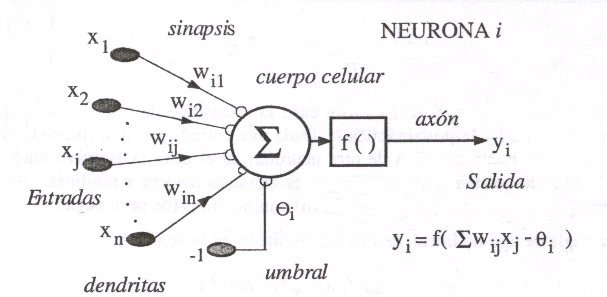
\includegraphics[width=80mm]{neurona_artif.jpg} \label{i_artifneuron}}
		\subfigure[Biológica]{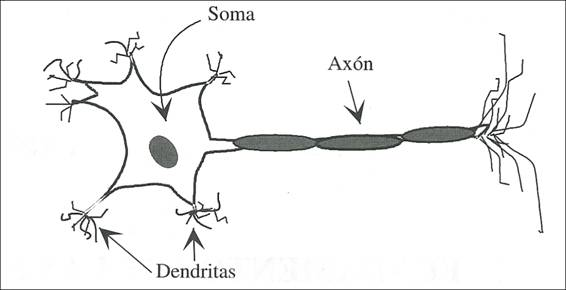
\includegraphics[width=80mm]{neurona_bio.jpg} \label{i_bioneuron}}
		\subfigure[Activacion]{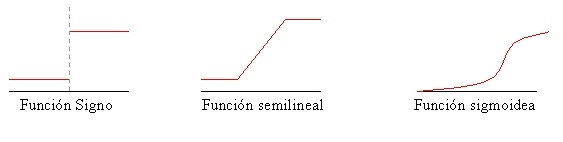
\includegraphics[width=100mm]{funcionesActivacion.jpg} \label{i_activacion}}
		\subfigure[Arquitectura]{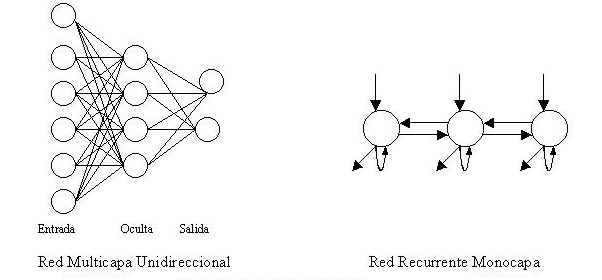
\includegraphics[width=100mm]{arquitectura.jpg} \label{i_arquitectura}}
		\caption{Modelos de neuronas \label{f-lenete-uml}}
	\end{figure}	
	
	\subsection{Red Neuronal Artificial} 
		Una red neuronal artificial (RNA) se puede definir (Hecht – Nielssen 93) como un grafo dirigido con las siguientes restricciones:	
		\begin{multicols}{2}
		 \begin{itemize}
		 	\item Los nodos se llaman elementos de proceso (EP).
		    \item Los enlaces se llaman conexiones y funcionan como caminos unidireccionales instantáneos
		    \item Cada EP puede tener cualquier número de conexiones.
		    \item Todas las conexiones que salgan de un EP deben tener la misma señal.
		    \item Los EP pueden tener memoria local.
		    \item Cada EP posee una función de transferencia que, en función de las entradas y la memoria local produce una señal de salida 
		    y / o altera la memoria local.
			\item Las entradas a la RNA llegan del mundo exterior, mientras que sus salidas son conexiones que abandonan la RNA.

			 \end{itemize}
		 \end{multicols}
	\subsection{Tipos de arquitectura de las RNA}
		 La arquitectura de una RNA es la estructura o patrón de conexiones de la red. Es conveniente recordar que las conexiones sinápticas son
		 direccionales, es decir, la información sólo se transmite en un sentido.
		 
		En general, las neuronas suelen agruparse en unidades estructurales llamadas capas. Dentro de una capa, las neuronas suelen ser del mismo 
		tipo. Se pueden distinguir tres tipos de capas:
		\begin{multicols}{2}
			\begin{itemize}
		 		\item De entrada: reciben datos o señales procedentes del entorno.
		 	   \item De salida: proporcionan la respuesta de la red a los estímulos de la entrada.
		   	 \item Ocultas: no reciben ni suministran información al entorno (procesamiento interno de la red).
		 	\end{itemize}
		\end{multicols}
		Generalmente las conexiones se realizan entre neuronas de distintas capas, pero puede haber conexiones intracapa o laterales y conexiones de
		realimentación que siguen un sentido contrario al de entrada-salida.
		
	\subsection{Aprendizaje de las RNA}
		 Es el proceso por el que una RNA actualiza los pesos (y, en algunos casos, la arquitectura) con el propósito de que la red pueda llevar a 
		 cabo de forma efectiva una tarea determinada.
		 Hay tres conceptos fundamentales en el aprendizaje:
		 \begin{multicols}{2}
			\begin{itemize}
		 		\item \textbf{Paradigma de aprendizaje:} información de la que dispone la red.
		 	   	\item \textbf{Regla de aprendizaje:} principios que gobiernan el aprendizaje.
		   		 \item \textbf{Algoritmo de aprendizaje:} procedimiento numérico de ajuste de los pesos.
		 	\end{itemize}
		\end{multicols}
		Existen dos paradigmas fundamentales de aprendizaje:
		\begin{multicols}{2}
			\begin{itemize}
		 		\item \textbf{Supervisado:} la red trata de minimizar un error entre la salida que calcula y la salida deseada (conocida), 
		 			de modo que la salida calculada termine siendo la deseada.
		 	   	\item \textbf{No supervisado o auto rganizado:} la red conoce un conjunto de patrones sin conocer la respuesta deseada. 
		 	   		Debe extraer rasgos o agrupar patrones similares.
		 	\end{itemize}
		\end{multicols}
		En cuanto a los algoritmos de aprendizaje, tenemos cuatro tipos:
		\begin{multicols}{2}
			\begin{itemize}
		 		\item \textbf{Minimización del error:} reducción del gradiente, retropropagación, etc. La modificación de pesos está orientada 
		 			a que el error cometido sea mínimo.
		 	   	\item \textbf{Boltzmann: }para redes estocásticas, donde se contemplan parámetros aleatorios.
		 	   	\item \textbf{Hebb:} cuando el disparo de una célula activa otra, el peso de la conexión entre ambas tiende a reforzarse (Ley de Hebb).
		 	   	\item \textbf{Competitivo:} sólo aprenden las neuronas que se acercan más a la salida deseada.
			\end{itemize}
		\end{multicols}
		
		Los algoritmos, y en general el proceso de aprendizaje, son complejos y suelen llevar bastante tiempo computacionalmente hablando. 
		Su ventaja es que una vez ha aprendido, la red puede congelar sus pesos y funcionar en modo recuerdo o ejecución.
		 
		 		


\chapter{DESCRIPCIÓN DE ACTIVIDADES REALIZADAS}
\markboth{ACTIVIDADES REALIZADAS}{ACTIVIDADES REALIZADAS}
\thispagestyle{empty}
\newpage

	Acorde a las normas estipuladas en las metodologías usadas [\ref{XP} y \ref{poo}] se han seguido una serie de pasos para la correcta 
	y efectiva realización del proyecto. Pese a que, a primera vista, la metodología de desarrollo extremo muestra algunas diferencias marcadas 
	respecto a las tradicionalmente usadas (\textit{Cascada, V, Espiral, etc.}) en el desarrollo de sistemas, en esencia conserva muchos de 
	los puntos clave de estas, es el desarrollo mucho mas rápido y enfocado a generar los módulos por separado e
	integrarlos al sistema solo y únicamente, cuando cada uno haya pasado las pruebas unitarias correspondientes, eso, en resumen es lo que 
	la hace diferente de las otras.
	En este capitulo se detallan las diferentes actividades, que componen el desarrollo tanto modular como integral del sistema, es importante 
	notar que la naturaleza la metodología \textit{xTreme Programing} hace que sean ciertamente diferentes a las tradicionales.
\section{Análisis}
	Es importante recalcar que la planificación inicial partió desde un punto ya establecido, por decirlo de alguna forma, el proyecto ya contaba
	con una base inicial sobre la cual comenzar a trabajar, es por tanto importante tener en cuenta que la dirección a seguir ya había sido definida.
	
	Sin embargo la falta de documentación hicieron difícil el saber con exactitud como proceder, razón por la cual se tuvo la necesidad de hacer 
	un nuevo análisis, partiendo de la idea central del proyecto, para ello una de las primeras cosas que se realizaron y, quizá una de las más
	importantes fue buscar si había o no, una solución parecida en el mercado, el resultado fue que pese a que actualmente existen en el medio
	soluciones que proveen diferentes formas de accesibilidad, estas están lejos de afrontar el problema desde una solución parecida a la que se 
	propone en el presente documento.
	
	Posterior a eso se procedió a identificar las principales características necesarias para la construcción de la solución propuesta.\\
	Las cuales de dividen en dos grandes áreas:
	\subsection{Requisitos funcionales \label{funcionales}}
		En términos simples nos referimos a este tipo de requerimientos como \textit{aquellos que permiten la interacción directa del usuario
		con la interfaz, su funcionalidad y en forma breve las funciones del sistema}, si nos referimos al capítulo (\ref{generalidades}) sección
		(\ref{objetivos}) donde se describen de forma precisa los resultados esperados, es posible definir los elementos funcionales que se requieren.
		
		\begin{enumerate}
			\item Debe existir una panel de configuración dentro de la cual encontrar las siguientes herramientas:
				\begin{itemize}
					\item Selección de la cámara a usar.
					\item Calibración de la cámara (\textit{webcam}).
					\item Entrenamiento del sistema.
				\end{itemize}
		\item El seguimiento de la dirección de la mirada debe ser transparente al usuario.
			\item La amplificación de la pantalla debe ser fluida y sin saltos bruscos.
			
		\end{enumerate}
		
		Es claro que el nivel de interacción con el usuario a nivel de interfaz, es mínimo, la naturaleza del sistema lo hace ser mas una 
		aplicación de asistencia.
		
	\subsection{Requisitos no funcionales \label{nofuncionales}}
		En esta sección se describen las funcionalidades que si bien forman parte integral del núcleo funcional del sistema, sí presentan una más
		interacciones con el o determinan en cierta medida el funcionamiento del mismo.\\
		Entre las que podemos encontrar las siguientes:
		\begin{description}
			\item[Interacción con el usuario:]\
				\begin{itemize}
					\item La aplicación una vez instalada debe ser transparente al usuario, es decir funcionar en segundo plano.
					\item La única interacción directa constate sera a través de los ojos.
				\end{itemize}
			\item[Requisitos de Hardware \& Software:] los siguientes son las características mínimas con las cuales debe de contar la máquina 
				en que se instale la aplicación: \
				\begin{multicols}{2}
					\begin{itemize}
						\item Sistema operativo Micrososft Windows \texttt{7/8.1/10}.
						\item Librerías de 32 bits.
						\item Procesador Quad Core o superior.
						\item 4Gb RAM.
						\item 1Gb de espacio en disco.
						\item Tarjeta gráfica dedicada \texttt{Nvidia GeForce}, preferentemente.
						\item Cámara web con resolución estándar.
					\end{itemize}
				\end{multicols}
			\item[Seguridad:]
				Dada la naturaleza de asistencia del sistema, entre las consideraciones de seguridad y dado que el manejo de datos sensibles 
				no existe, se considera solo lo siguiente:
				\begin{description}
					\item[Disponibilidad:] debe estar disponible mientras el equipo este encendido.
				\end{description}
			\item[Condiciones de iluminación:] para un funcionamiento aceptable las condiciones de iluminación del entorno son importantes, 
			la siguiente lista  contempla las principales a tener ene cuenta:
			\begin{multicols}{2}
				\begin{itemize}
					\item Fuentes intensas de luz detrás del usuario.
					\item Oscuridad total o parcial.
					\item Cambios bruscos de luz.
				\end{itemize}
				\end{multicols}
			Estas son solo recomendaciones en cuanto al entorno de operación, con el único objetivo de aumentar el rendimiento y confiabilidad.
		\end{description}
		Las características tanto internas del sistema como las externas, son las mínimas consideradas para tener un sistema funcional que cunmpla con 
		los objetivos planteados, cumplir con todos los puntos es por tanto algo que no se puede evitar a fin de conseguir un resultado aceptable en la
		siguiente etapa.

\newpage
\section{Diseño}
	Definidos los requerimientos, se deben generar un diseño que permita cumplir, de forma precisa todos los elementos que correspondan a 
	al núcleo de la aplicación, así como los sub-sistemas periféricos.
	\subsection{Aproximación clásica \label{clasica}}
		Una primera aproximación tomando como base el trabajo que ya existía al momento de tomar el proyecto fue, por decirlo de alguna forma una aproximación 
		clásica, fundamentada de lleno en la segmentación de imágenes por métodos convencionales, extracción y detección de características por medio de 
		cálculos matemáticos y segmentación de imágenes, la siguiente imagen (\ref{f_clasic}) ilustra claramente este enfoque\\
		\begin{figure}[t]
		 	\centering
		 	\subfigure[Clásico]{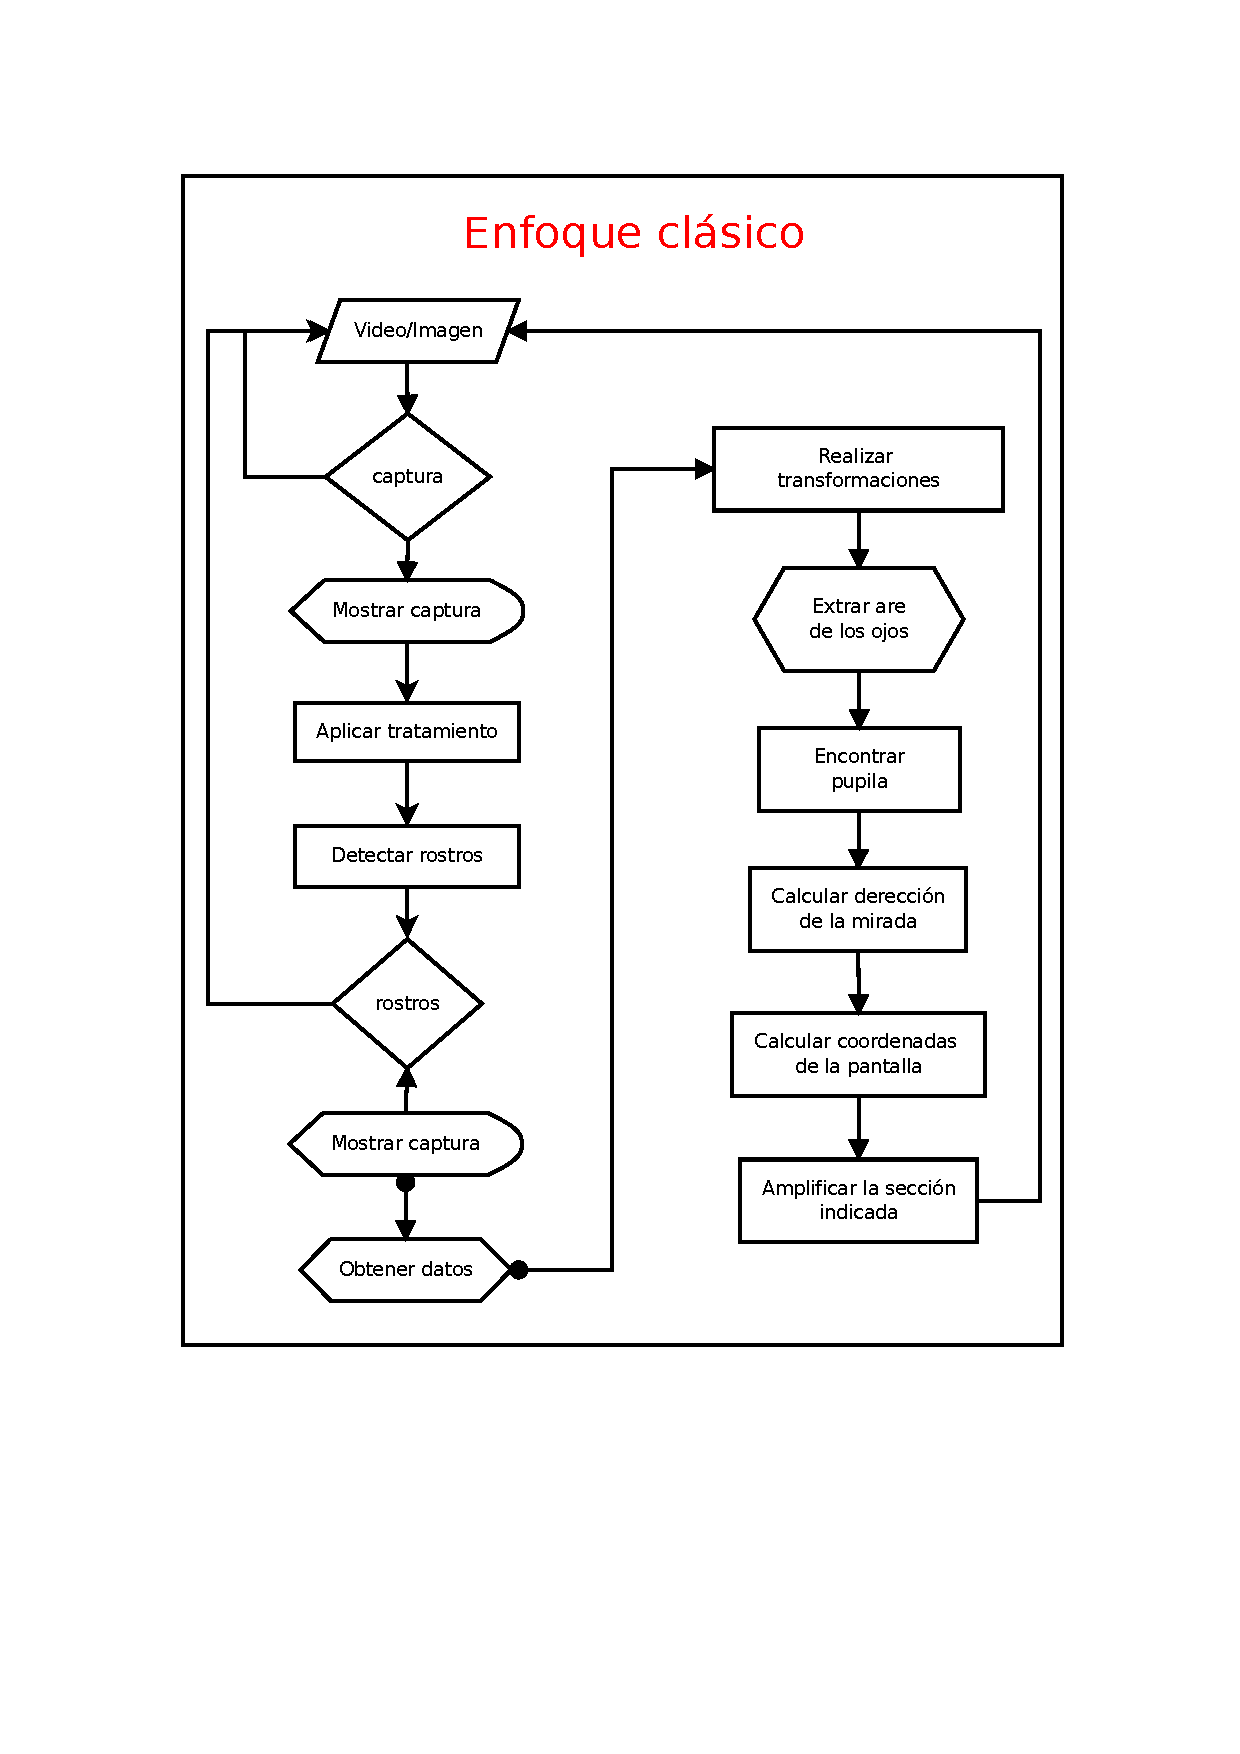
\includegraphics[width=69mm]{./Diagramas/clasico.pdf} \label{f_clasic}}
		 	\subfigure[LeNet]{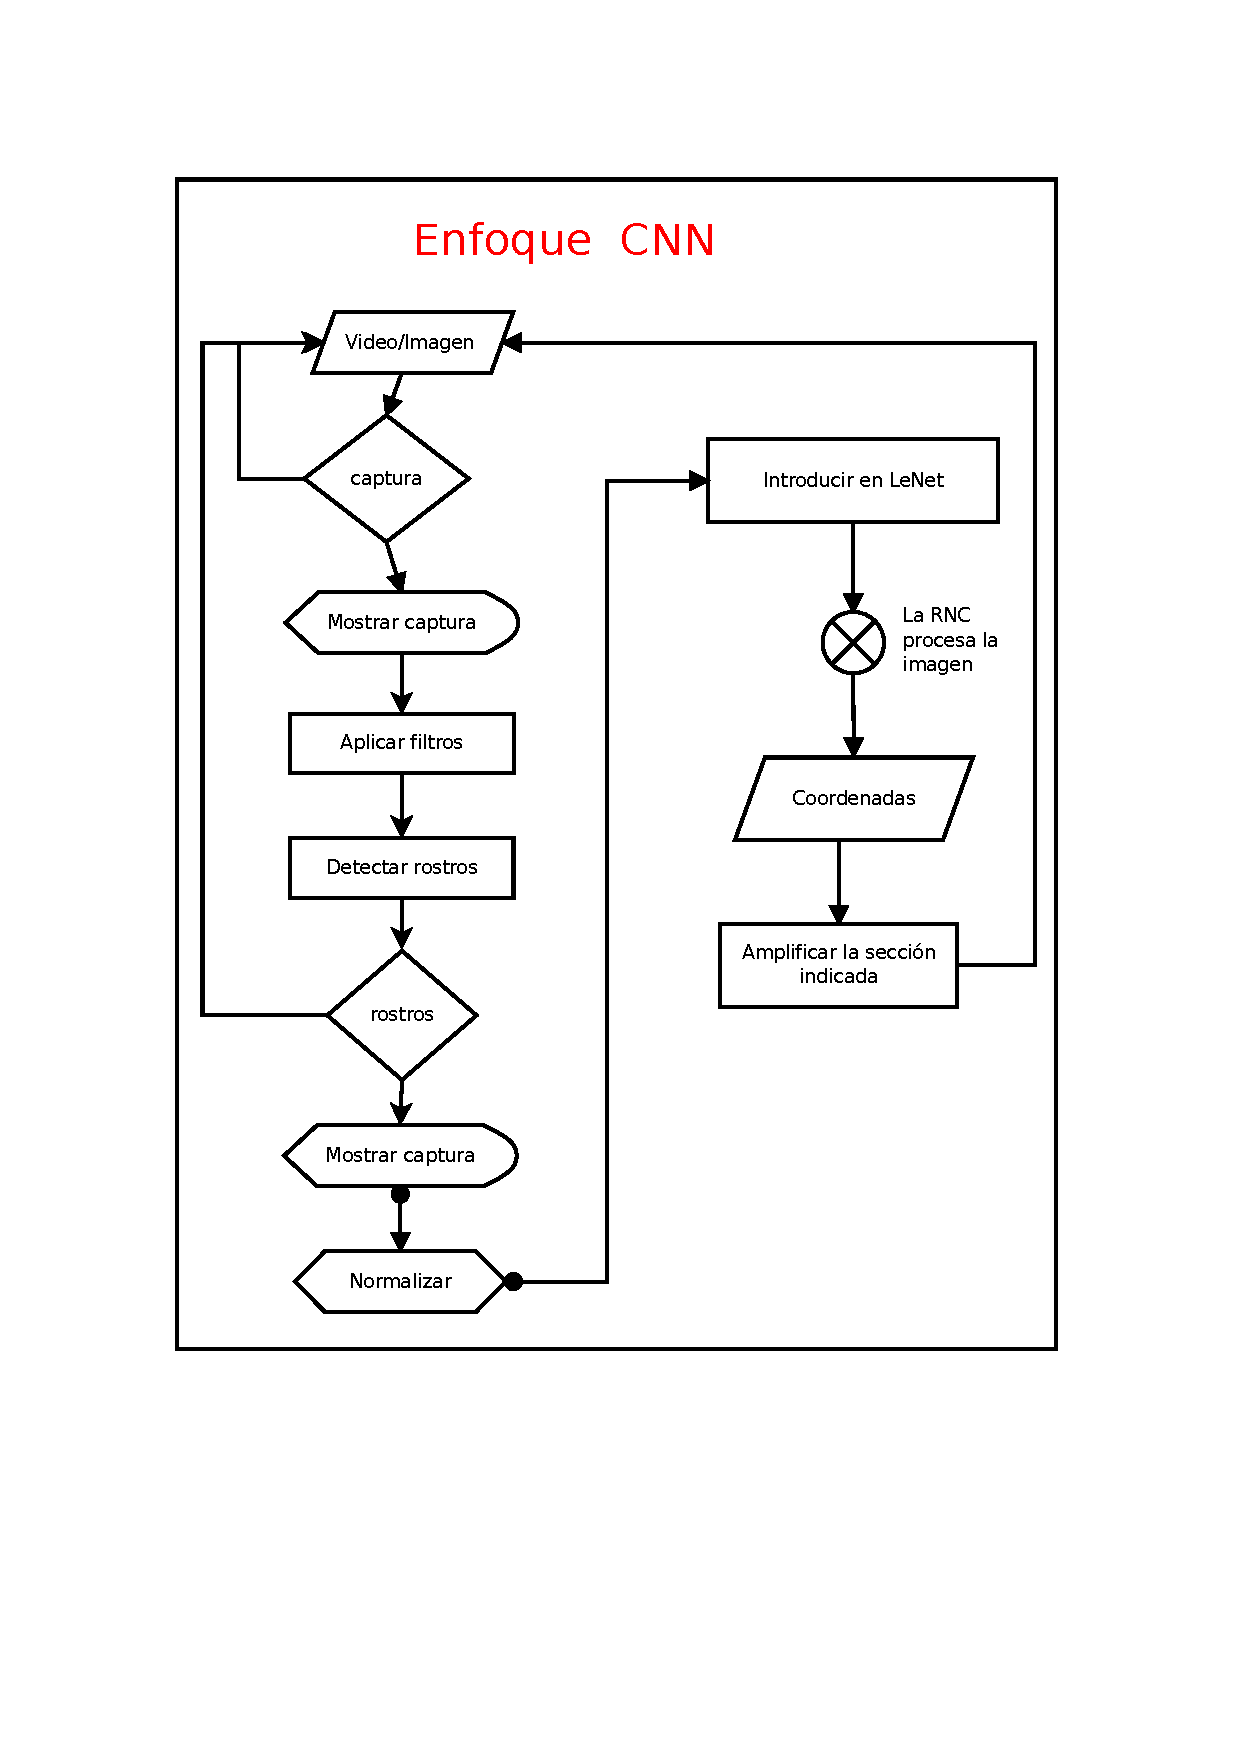
\includegraphics[width=69mm]{./Diagramas/cnn.pdf} \label{f_lenet}}
			\caption{Los dos diferentes enfoques considerados a) Clasico b) LeNet} 
			\label{fig:enfoque_clásico}
		\end{figure}
	\subsection{Aproximación por Red Neural convolucional \label{lenet}}
		Sin embargo la solución clásica, nos es optima en condiciones no controladas, es decir fuera de las condiciones de un laboratorio, este método 
		presenta rendimientos con niveles de precision bajos, las condiciones de iluminación, resolución, distancia a la cámara, etc., repercuten en el 
		proceso de identificación de la dirección de la mirada.\\
		Investigando maneras de reducir este problema y obtener un sistema mucho mas robusto y confiable, se descubrió una forma de afrontar el proyecto que
		hasta este punto no se había considerado: \textsf{redes neuronales}.
		\footnote{\scriptsize Encontrará más información al respecto en el Apéndice A [\ref{a-neuronales}].}\\
		\subsubsection{Diseño de objetos.}		
			En la imagen [\ref{f_lenet}] se muestra el diseño del enfoque basado en esta aproximación, como se puede observar el es prácticamente igual,
			al menos hasta la parte de la adquisición y reconocimiento del rostro, una ves obtenidos, el proceso cambia radicalmente pues la técnica
			para determinar la dirección de la mirada se hace usando las capacidades de las redes neuronales convolucionales (\texttt{RNC}) como 	
			en la figura [\ref{f-cnn}].
			\begin{figure}
			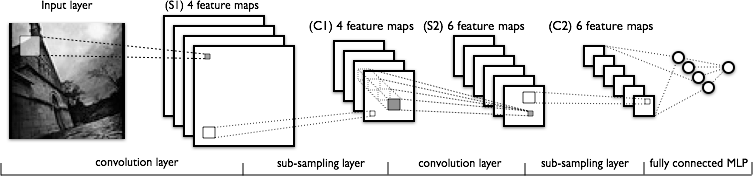
\includegraphics[width=140mm]{mylenet.png}
			\caption{Ejemplo de una red neuronal convolucional \label{f-cnn}}
			\end{figure}
			
			Este modelo presenta enormes ventajas sobre el clásico, la capacidad de adaptarse a diferentes condiciones, hacen que las redes neuronales sean
			la forma más confiable de abordar el problema.
			\begin{figure}[t]
				\centering
				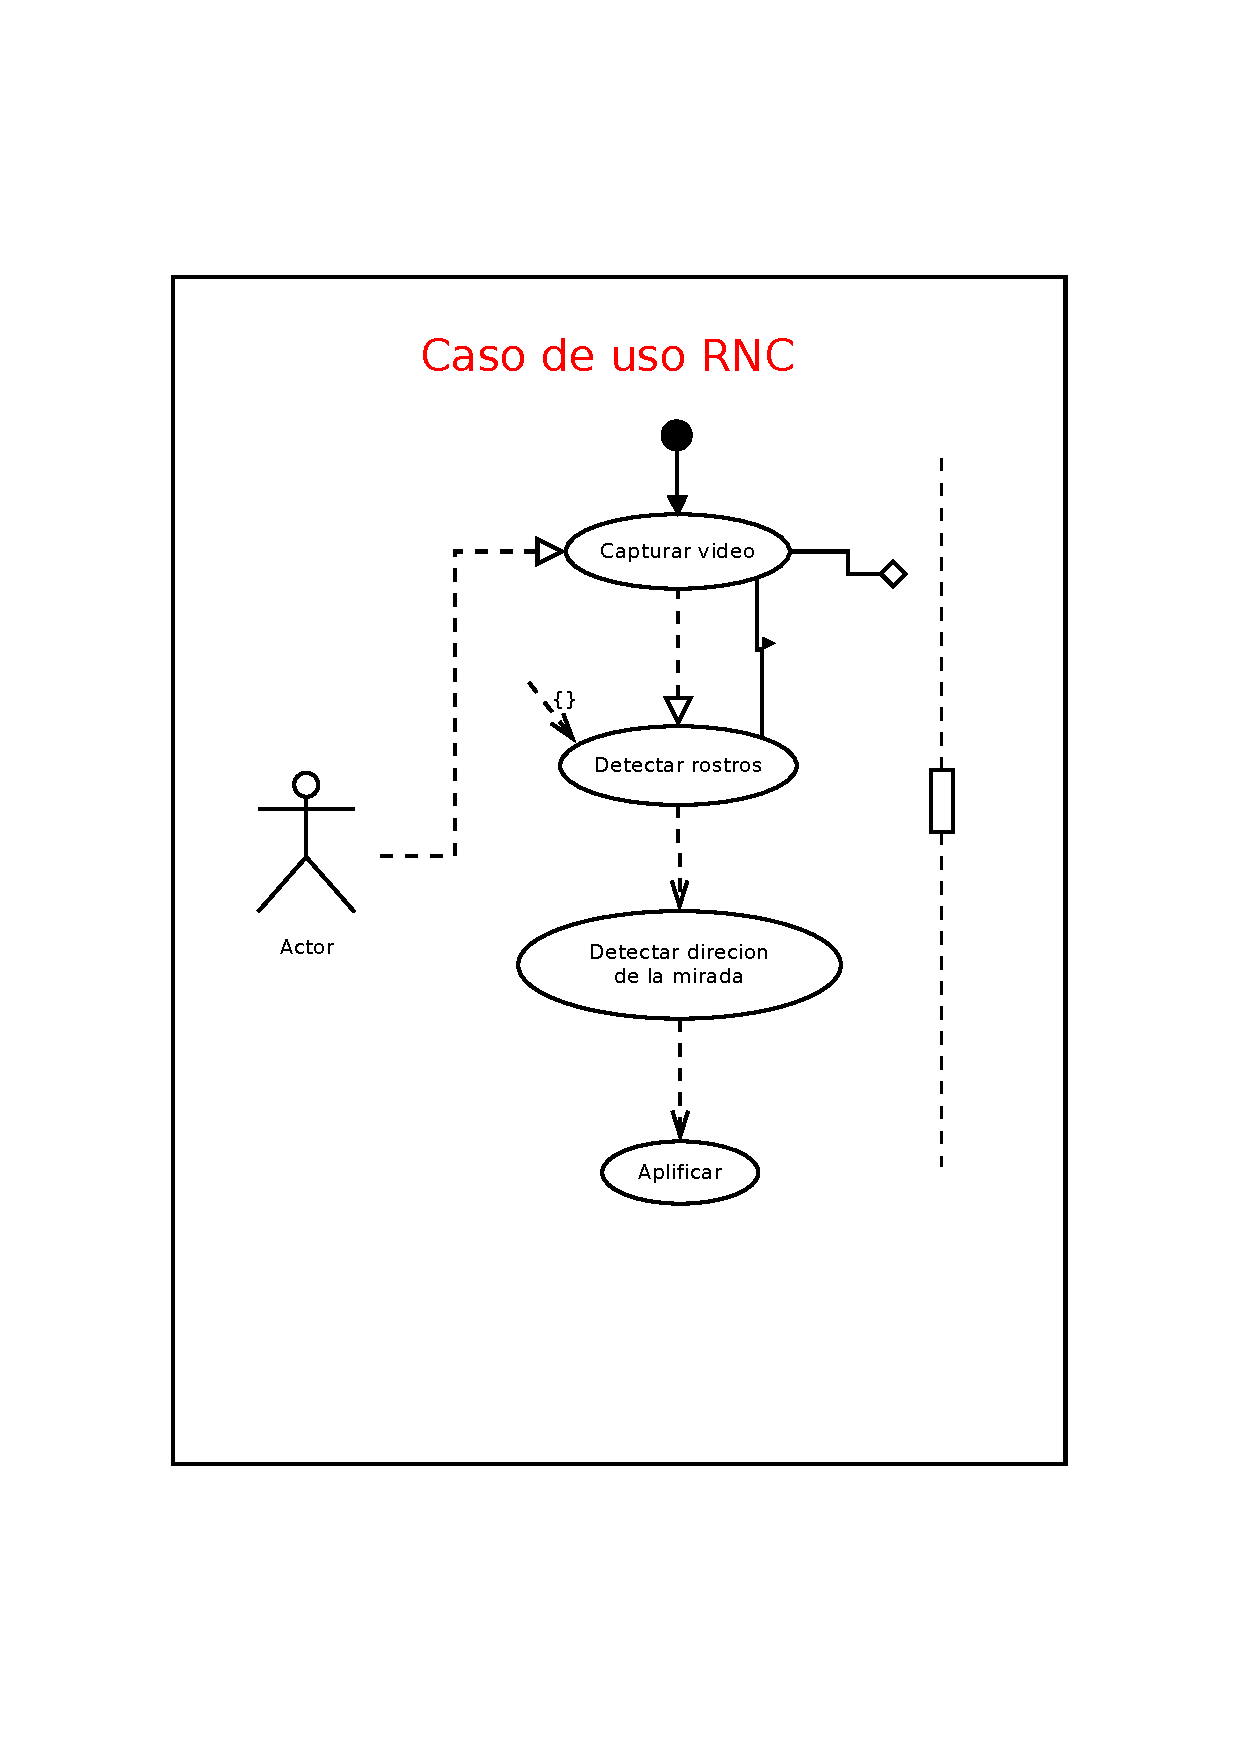
\includegraphics[width=50mm]{./Diagramas/caso_uso_lenet.pdf} \label{f_uml_lenet}
				\caption{Diagramas de caso de uso. \label{f-lenete-uml}}
			\end{figure}	
			El diagrama [\ref{f-lenete-uml}] ilustra el modelo de interacción entre el usuario (\textit{actor}) y el sistema.
		
		\subsubsection{Diseño de interfaces}
			La cantidad de interfaces con las que cuenta el sistema se reduce a una, por simplicidad y facilidad ésta no cuenta con interfaz gráfica,
			es un pequeño menú en la ventana de símbolos del sistema (\texttt{CMD}), con tres opciones:
			\begin{itemize}
				\item \textbf{Iniciar:} inicia el sistema.
				\item \textbf{Calibrar} se encarga de obtener ciertos parámetros de la cámara.
				\item \textbf{Salir.}
			\end{itemize}
			En la etapa actual no es necesario que el usuario cuente con más opciones, pues dada la forma en que se procesara la información dentro 
			de la red neuronal, el usuario realmente no necesita controlar los parámetros que esta usa para su funcionamiento.\\
			
		Definida la forma en la que se van a interactuar los componentes internos del sistema y la interacción con el usuario y el usuario, solo queda, 
		construir el sistema.
		
\newpage
\section{Desarrollo}
	En esta fase del desarrollo y definidas las características, requerimientos y diseñados los modelos, la construcción  cada una de esas piezas 
	que integran el sistema se debe hacer de forma que cumpla con cada una de ellas. Si nos referimos a la metodología POO y XP de la secciones 
	[\ref{XP}] y [\ref{poo}], recordaremos pues que este proceso, incluidos los dos anteriores, los estaremos aplicando iteración, tras iteración, 
	modulo tras modulo. La razón por la que en este documento no se ha incluido de forma explicita el proceso para cada uno de los módulos, es 
	precisamente por eso, cada una de las piezas que componen el sistema se ha construido por separado, básicamente, solo una parte de todo
	el sistema se ha mantenido en cada fase, y esa es la parte encargada de realizar la captura de vídeo desde la cámara web y la detección de 
	rostros en cada cuadro obtenido, esto haciendo uso de las librerías \texttt{IntraFace}[\ref{intraface}] y \texttt{OpenCV}[\ref{cv}].\\
	
	Las siguientes secciones tratan en mayor profundidad el desarrollo de los diferentes componentes del sistema.
	
	\begin{figure}[t]
		\centering
		\subfigure[Vídeo]{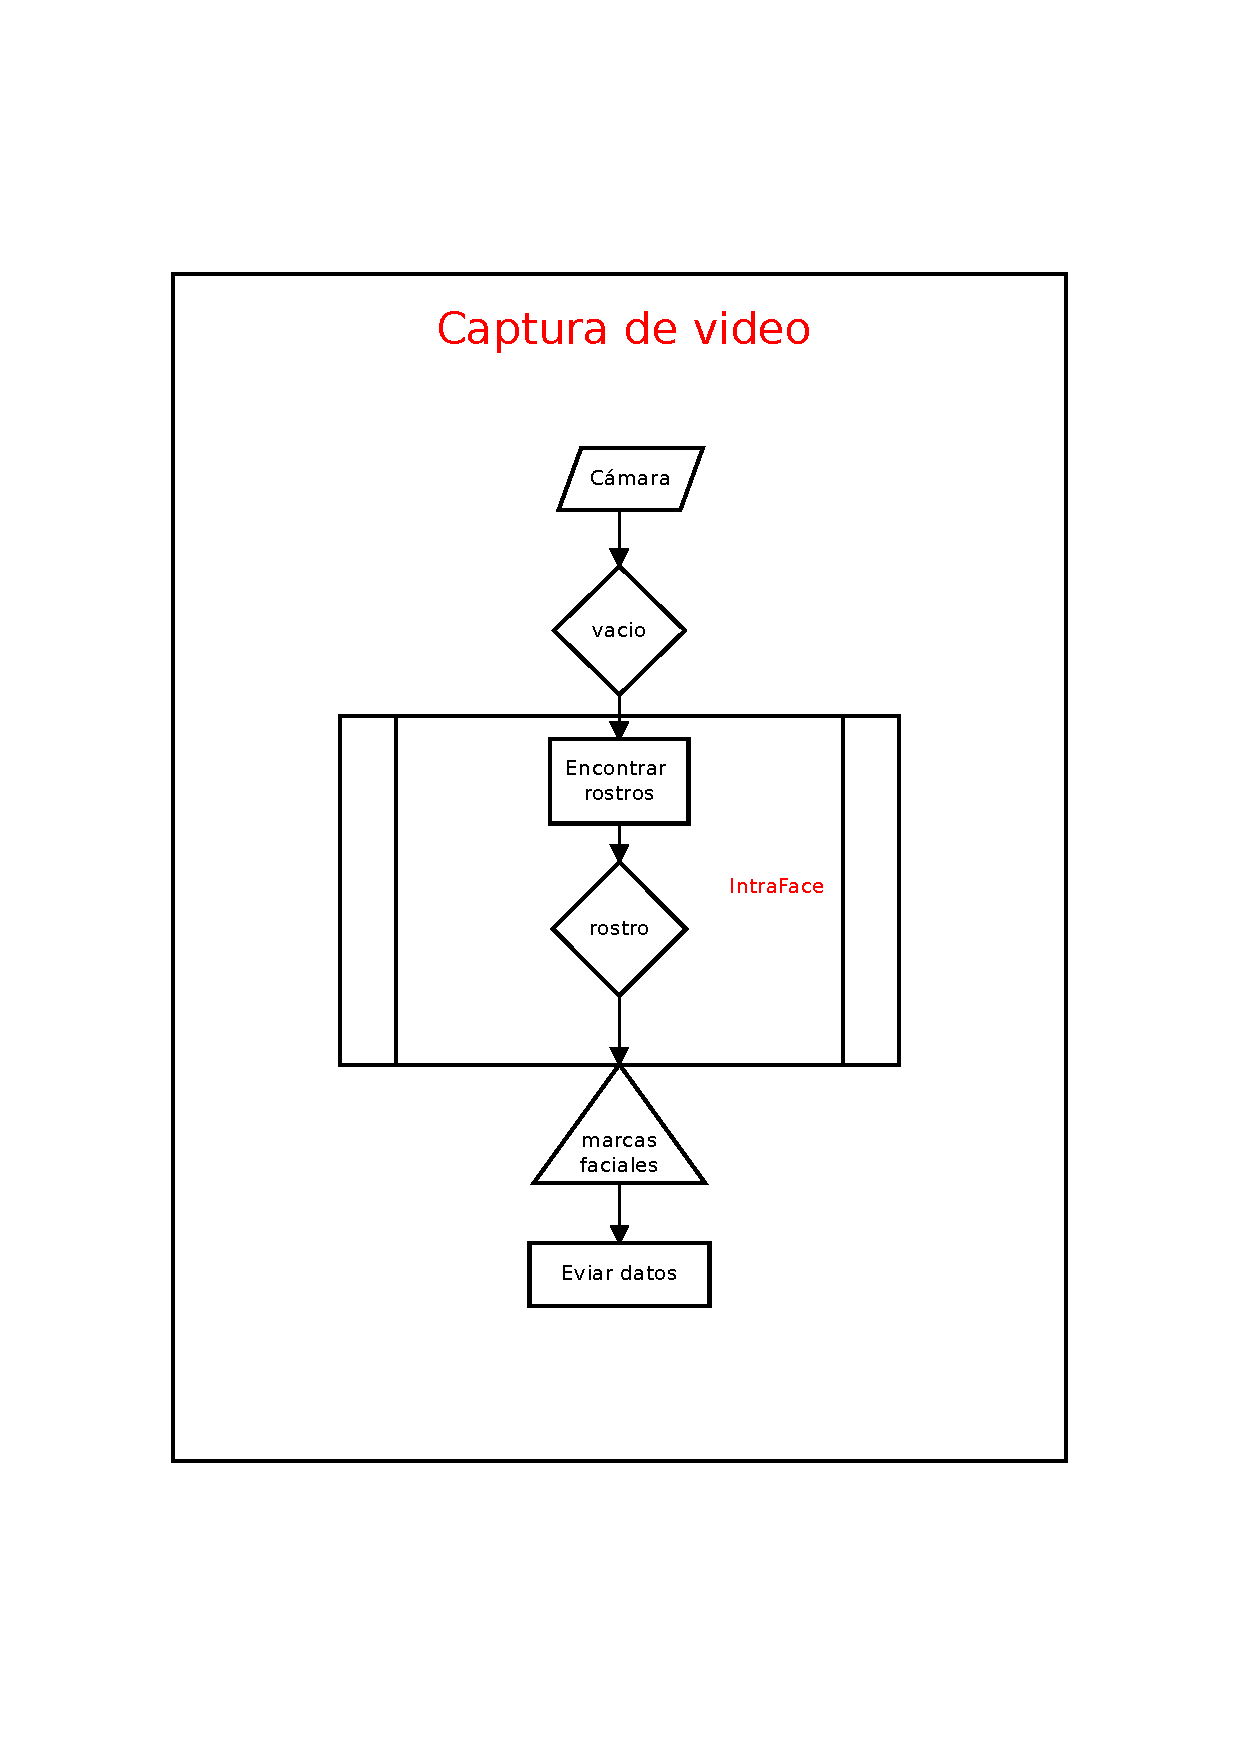
\includegraphics[width=60mm]{./Diagramas/video.pdf} \label{f_uml_video}}
		\caption{Diagramas de flujo, diseño. \label{f-lenete-uml}}
	\end{figure}	
	\subsection{Captura de vídeo y detección de rostros}
		Este modulo es el encargado de generar el flujo de entrada del sistema, comprobando la disponibilidad de la cámara, y el posterior 
		procesado para el reconocimiento de rostros en cada uno de los cuadros capturados.
		
		Básicamente lo que hace este modulo es toma un cuadro del stream del vídeo y lo analiza usando IntrFace, la librería retorna varios
		datos:
		\begin{multicols}{2}
			\begin{enumerate}
				\item Orientación de la cabeza en el espacio 3D, \textit{en ángulos de Euler} \texttt{Roll, Yaw, Pitch}.
				\item Un conjunto de marcadores faciales, entre los que se encuentran seis coordenadas (x,y) para cada ojo.
				\item La cantidad de rostros detectados y la zona de la pantalla en la cual esta cada uno.
			\end{enumerate}
		\end{multicols}
		Con todos estos datos es posible hacer recortes de la imagen en general y extraer regiones de interés, que en este caso son el 
		área  de los ojos y los datos sobre la orientación de la cabeza.
		Los cuales son enviados posteriormente a diferentes clases para seguir el proceso.

	\subsection{Clasificador de parpadeos}
		La construcción de este modulo no fue planeada e un inicio, y por ello no forma parte de los requerimientos, sin embargo
		durante el proceso de adquisición de imágenes se hizo necesario el discriminar entre capturas utilizables y aquellas que no.
		La idea básica es determinar cuando el ojo esta abierto y cuando esta cerrado, 
		
	\subsection{Normalizar imágenes}
		Antes de enviar las imágenes a la red neuronal \texttt{LeNet} para obtener la dirección de la mirada, es necesario realizar un 
		tratamiento previo de las mismas, a fin de lograr los mejores resultados.
		Basicamnete lo que se hace como en \cite{Sugano}, en resumen lo que se hace es normalizar tanto la imagen como la posición de 
		la cabeza dentro del espacio de los ángulos polares. 
		Para hacerlo, y entendiendo que fundamentalmente la posición de un objeto tiene seis grados de libertad, en el caso de querer 
		estimar la dirección de la mirada el estimador debe hacerlo considerando cambios en 6D espaciales.
		Poro no toda esa información es necesaria, el estimador al final solo necesita dos grados de libertad, algo que se logra escalando 
		y rotando la imagen a fin de compensar la perspectiva de la imagen, de forma que:
		\begin{enumerate}
			\item La cámara enfoque el punto medio entre los ojos desde una determinada distancia.
			\item Hacer paralelos los ejes \textit{x}, en el espacio de coordenadas de la cabeza y de la cámara 
			\item Recortar las secciones de lo ojos con una misma resolución \textsf{W x H} y una distancia focal en el espacio de normalizado
				de la cámara.
		\end{enumerate}
		El resultado sera un conjunto de imágenes con una resolución estándar y un vector 2D de los ángulos de la cabeza (\textit{Yaw y Pitch)}.
		De esta forma los valores reales de la posición de la mirada son convertidos al espacio normalizado en 2D de la cámara.
		Para reducir el efecto de las condiciones de iluminación el histograma de las imágenes es equializado antes del procesos de normalizar.
	\begin{figure}[t]
		\centering
		\subfigure[Max Pooling]{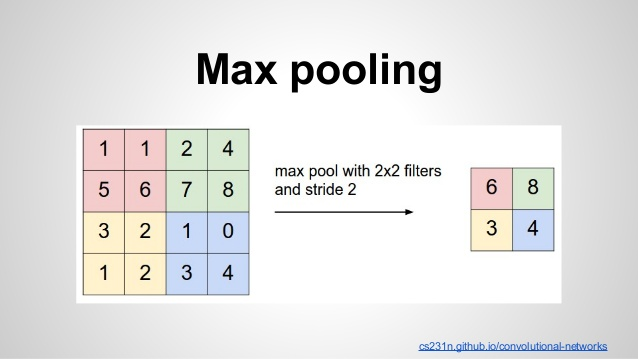
\includegraphics[width=80mm]{max_pooling.jpg} \label{i_pooling}}
		\subfigure[LeNet]{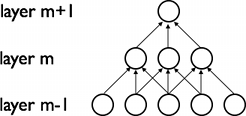
\includegraphics[width=80mm]{lenet_model.png} \label{i_lenetModel}}
		\subfigure[Tipica CNN]{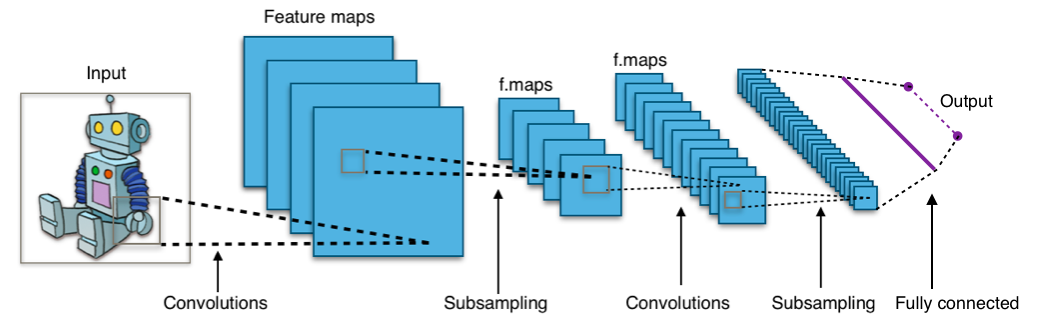
\includegraphics[width=100mm]{typical_cnn.png} \label{i_typical_cnn}}
		\caption{Pooling \& LeNet \label{f-lenete-uml}}
	\end{figure}	
	\subsection{Procesado}
		La tarea de la CNN es aprender a extraer de los datos entradas (\textit{posición de la cabeza e imágenes de los ojos}, el angulo de la
		mirada en el espacio normalizado.
		Para lograr eso es el modelo usado es la arquitectura de red \texttt{LeNet} \ref{i_lenetModel} que consiste en una capa de convolución 
		seguida de una capa 	de \textit{max-pooling} \ref{i_pooling}, una segunda capa de convolución y otra capa max-pooling, finalmente una 
		capa totalmente conectada.
		Una representación de esto la podemos ver en la imagen [\ref{i_typical_cnn}].
		Se entreno una un regresor lineal sobre la capa totalmente conectada para predecir el vector del angulo de la mirada. Se uso una 
		CNN multimodal, con eln de obtener ventaja de ambas imágenes de los ojos y la orientación de la cabeza.
		La dirección dela mirada fue agregada a la salida de la capa totalmente conectada.
		Las imagenes de entrada son de \textit{60 x 36 pixeles} en escala de grises, para las dos primeras capas convolucionales el tamaño
		es de\textit{5 x 5 pixeles}, mientras que el número de características es de 20 para la primera y 50 para la segunda. El número de 
		neuronas en la capa oculta es de 500, y cada una de ellas esta conectada a las características encontradas en la capa convolucional 
		anterior y es calculada por la sumatoria de todos los valores de activación. La salida de la res es un vector \textit{g} 2D 
		con los dos ángulos de la mirada \textit{yaw y Pitch}. Como función de error se usa la sumatoria de los errores individuales en la
		medida de la distancias entre la predicción de g y el vector de ángulos actuales g.
		
	\subsection{Amplificación}
		Una 	vez que las CNN nos entrega el vector con los ángulos de la mirara, estos son convertidos a una coordenada aproximada en 
		el sistema de de la pantalla en cuestión, una vez hecho ese paso, lo único que resta es llamar a la API de maginificación de 
		Microsoft Windows y pasar como parámetros la coordenada (\textit{X, Y}) estimada del vector 2D g.
		El resultado es una ventana que muestra la sección de la pantalla
	
\newpage	
\section{Pruebas}
	Las pruebas realizadas hasta el momento aun no se aplican al sistema completo, en el estado actual de desarrollo solo se han hecho pruebas
	unitarias para cada uno de los módulos, de acuerdo a la metodología, cada uno de ellos fue agregado al sistema solo cuando su comportamiento 
	cumplió las  especificaciones iniciales.
	
	Una vez terminada de construir e implementar la rede neuronal con el resto de los componentes se incluirán los resultados de las pruebas de 
	rendimiento.
	

\section{Conclusiones}
	Divertido e interesante, si tuviera que definir lo que este proyecto ha sido para mi, esas serian las palabras que elegiría.
	Obviamente hay muchas cosas más que me ha dejado, la cantidad de aprendizaje ha sido monumental, comenzado por la que es quizá la lección más
	importante, me ha quedado claro que no debo subestimar la complejidad de un problema solo por que en la teoría y en la definición de los 
	objetivos, suene y parezca algo fácil, mi asesor de \texttt{CICATA} me contó una historia  al inicio de la estadía que mas o menos va así:\\
	\textit{En alguna universidad por los 50's, un alumno y un profesor platicando sobre el tema de visión artificial, salio pues el tema de 
	como hacer posible que las máquinas puedan ver el mundo, el alumno subestimando el problema dijo al profesor que esperara, que el construiría
	esa máquina, a día de hoy es algo que aun no logra hacer, las dificultades encontradas son grandes, pese a la simplicidad aparente de la tarea.}\\
	
	Creo que con algo de pena debo decir que he cometido el mismo error de ese estudiante, subestime el problema al inicio, al final me di cuenta 
	que de haber abordado el problema con la responsabilidad que lo hago ahora, hubiese logrado resultados mucho más allá de los planteados.
	
	Por otro lado, es muy interesante ver como el modelo de aproximación que se implemento, es parte de una de las ramas de la tecnología que 
	presenta actualmente un panorama muy prometedor en la industria de la información, las capacidades de calculo actuales son por primera vez, aptas
	para llevar la potencia de calculo de los métodos aplicados, al usuario común.
	El panorama que se ha abierto ante mi es alentador, me descubro a mi mismo, este será el camino que seguiré en mi linea de especialización.
	
	Como último debo agradecer al Dr. Joaquín, mi asesor interno por parte de CICATA, pues de alguna forma despertó en mi el interés por seguir 
	preparándome, y quien sabe, es posible que el próximo semestre este aquí comenzando la maestría.
	

\chapter*{Resultados}
\markboth{}{}
\thispagestyle{empty}
\lhead[\thepage]{}
\rhead[]{\thepage}
\addcontentsline{toc}{chapter}{Apendice}
\newpage

\chapter*{Conclusiones y recomendaciones}
\markboth{}{}
\thispagestyle{empty}
\lhead[\thepage]{}
\rhead[]{\thepage}
\addcontentsline{toc}{chapter}{Apendice}
\newpage



			

\newpage

%----------------------------------------------------------------------------------------
%	BEGIN GLOSARIO
%----------------------------------------------------------------------------------------			
\newpage
\printnoidxglossaries
\pagenumbering{roman}
%----------------------------------------------------------------------------------------
%	END GLOSARIO
%----------------------------------------------------------------------------------------
%---------------------------------------------------------------------------------------
%	BIBLIOGRAPHY
%----------------------------------------------------------------------------------------

\begin{thebibliography}{99} % Bibliography - this is intentionally simple in this template

\small
\bibitem{IngSoft}{\textbf{Ian Sommerville}},
Ian Sommerville, María Isabel Alfonso Galipienso
[\textit{ingeniería del software, Séptima edición.}]. 
Pearson Educación.S.A., Madrid, 2005. ISBN: 84-7829-074-5

\bibitem {EProg}{\textbf{Beck}}
Kent Beck 
[\textit{"Extreme Programming Explained: Embrace Change"}],
Addison-Wesley Pub Co; ISBN: 0201616416, 1"a Edición octubre 1999

\bibitem{rdev} {\textbf{Development Core Team (2008)}}. 
R Foundation for Statistical Computing, 
[\textit{R: A language and environment for statistical computing.}]
Vienna, Austria. ISBN 3-900051-07-0, \href{http://www.R-pro ject.org}{http://www.R-pro ject.org}

\bibitem{artR}{\textbf{Santana Sepúlveda, Julio Sergio}}.
Julio Sergio Santana Sepúlveda y Efraín Mateos Farfán.
[\textit{El arte de programa en R: un lenguaje para la estadística.}]
México: Instituto Mexicano de Tecnología del Agua, UNESCO, 2014. SBN: 978-607-9368-15-9

\bibitem{Sugano}{\textbf{Y.Sugano}}
Y.Sugano, Y. Matsushita and Y. Sato.
[\textit{Learning-by-sythesis for appeareance-based 3d gaze estimation.}]
In Proc. CVR, pages 1821-1828, 2014, 1,2,3,4,5,6,7,8.


\bibitem{python}{\textbf{Rául Gonzáles Duque}},
Rául Gonzáles Duque
[\textit{Python para todos.}]
Este libro se distribuye bajo una licencia Creative Commons Reconocimiento 2.5 España

\bibitem{OOD}{\textbf{David}}
David E.Brumbaugh
[\textit{Object-Oriented Developement with C++}]. 
Edt.Wile, 1994.


\bibitem {xProgv}{\textbf{Fowler}}
Martin Fowler 
[\textit{Variations on a Theme of XP}], 
\href{http://www.martinfowler.com/articles/xpVariation.html}{http://www.martinfowler.com/articles/xpVariation.html}

\bibitem{EvoProg} {\textbf{Harrison}}
Peter Harrison 
[\textit {Evolutionary Programming}],
\href{http://www.devcentre.org/research/evoprogramming.htm}{http://www.devcentre.org/research/evoprogramming.htm}


\end{thebibliography}


%----------------------------------------------------------------------------------------
 
\end{document}


